% ============================================================
% HSBI Beamer — ISLP Lecture Series — IMPROVED EDITION
% Chapter 2: Statistical Learning
% ============================================================
\documentclass[aspectratio=169,11pt]{beamer}
\usepackage[utf8]{inputenc}\usepackage[T1]{fontenc}\usepackage[english]{babel}
\usepackage{graphicx}\usepackage{booktabs}\usepackage{amsmath,amssymb,amsfonts}
\usepackage{mathtools}\usepackage{hyperref}\usepackage{xcolor}
\usepackage{verbatim}\usepackage{alltt}
\usepackage{tikz}\usetikzlibrary{calc,arrows.meta,positioning,shapes}
\usepackage{tcolorbox}\tcbuselibrary{skins}

\usetheme{Madrid}\usecolortheme{default}
\setbeamertemplate{navigation symbols}{}
\setbeamertemplate{footline}[frame number]
\setbeamertemplate{blocks}[rounded][shadow=false]
\setbeamertemplate{headline}{%
  \leavevmode\hbox{%
    \begin{beamercolorbox}[wd=\paperwidth,ht=2.2ex,dp=0.9ex]{section in head/foot}%
      {\fontsize{4.6}{5.2}\selectfont%
       \insertsectionnavigationhorizontal{\paperwidth}{}{\hskip0pt plus1filll}}%
    \end{beamercolorbox}}%
}
\setbeamerfont{section in head/foot}{size=\tiny}
\setbeamerfont{palette primary}{size=\tiny}
\setbeamerfont{palette tertiary}{size=\tiny}
\setbeamerfont{section in toc}{size=\footnotesize}

\usepackage{listings}
\definecolor{pyKw}{RGB}{0,0,180}\definecolor{pyStr}{RGB}{20,120,40}
\definecolor{pyCom}{RGB}{120,120,120}\definecolor{accent}{RGB}{38,70,140}
\lstdefinestyle{Pystyle}{language=Python,basicstyle=\ttfamily\footnotesize,
  keywordstyle=\color{pyKw}\bfseries,commentstyle=\color{pyCom}\itshape,
  stringstyle=\color{pyStr},showstringspaces=false,upquote=true,
  columns=fullflexible,breaklines=true,literate={~}{{$\sim$}}1}
\lstset{style=Pystyle}

\AtBeginSection[]{\begin{frame}{Outline}
  \begin{columns}[t]
    \begin{column}{0.5\textwidth}
      \tableofcontents[currentsection,sectionstyle=show/shaded,subsectionstyle=show/show/hide,sections={1-6}]
    \end{column}
    \begin{column}{0.5\textwidth}
      \tableofcontents[currentsection,sectionstyle=show/shaded,subsectionstyle=show/show/hide,sections={7-11}]
    \end{column}
  \end{columns}
\end{frame}}

\newcommand{\islpsource}[1]{%
  \vfill\hfill{\tiny\itshape\color{gray}Source: #1 \textemdash{} ISLP, James et al.\ (2023).}\par
}

\newtcolorbox{takeaway}[1][Takeaway]{enhanced,colback=green!4,colframe=green!50!black,
  boxrule=0pt,leftrule=2.5pt,arc=2pt,fonttitle=\bfseries,title=#1,
  left=2mm,right=2mm,top=1mm,bottom=1mm}
\newtcolorbox{numexample}[1][Worked example]{enhanced,colback=orange!4,colframe=orange!70!black,
  boxrule=0pt,leftrule=2.5pt,arc=2pt,fonttitle=\bfseries,title=#1,
  left=2mm,right=2mm,top=1mm,bottom=1mm}
\newtcolorbox{readme}[1][How to read this]{enhanced,colback=blue!4,colframe=accent,
  boxrule=0pt,leftrule=2.5pt,arc=2pt,fonttitle=\bfseries,title=#1,
  left=2mm,right=2mm,top=1mm,bottom=1mm}

\title{Quantitative Research Methods}
\subtitle{Chapter 2: Statistical Learning}
\author{Prof.\ Dr.\ Christoph Weisser}\institute{HSBI}
\date{Summer Semester 2026}\graphicspath{{images/}}

\newtcolorbox{exercise}[1][Exercise]{enhanced, fontupper=\footnotesize, colback=purple!4, colframe=purple!55!black, boxrule=0pt, leftrule=2.5pt, arc=2pt, fonttitle=\bfseries, title=#1, left=2mm, right=2mm, top=1mm, bottom=1mm}
\newtcolorbox{solutionbox}[1][Solution]{enhanced, fontupper=\footnotesize, colback=teal!5, colframe=teal!55!black, boxrule=0pt, leftrule=2.5pt, arc=2pt, fonttitle=\bfseries, title=#1, left=2mm, right=2mm, top=1mm, bottom=1mm}

% Reclaim ~2pt of body height (the custom nav headline makes full slides tip over by ~1.83pt)
\addtobeamertemplate{frametitle}{}{\vspace{-2pt}}

\newtcolorbox{longexercise}[1][Extended exercise (15 min)]{enhanced, fontupper=\footnotesize, colback=violet!6, colframe=violet!55!black, boxrule=0pt, leftrule=3pt, arc=2pt, fonttitle=\bfseries, title=#1, left=2mm, right=2mm, top=1mm, bottom=1mm}

\newtcolorbox{labnote}[1][Run this live in the lab notebook]{enhanced, fontupper=\footnotesize, colback=cyan!7, colframe=cyan!45!black, boxrule=0pt, leftrule=3pt, arc=2pt, fonttitle=\bfseries, title=#1, left=2mm, right=2mm, top=1mm, bottom=1mm}

\begin{document}
\begin{frame}[plain]\titlepage\end{frame}

\begin{frame}{The course at a glance}
  \footnotesize
  \begin{center}
  \begin{tabular}{@{}c r l@{}}
    & \textbf{Lecture} & \textbf{Topic}\\
    \midrule
     & 1 & Ch.\ 1 + 2 --- Introduction; what is statistical learning \\
    $\blacktriangleright$ & \textbf{2} & \textbf{Ch.\ 2 --- Accuracy, bias--variance, Bayes classifier, KNN} \\
     & 3--4 & Ch.\ 3 --- Linear regression (estimation, inference, diagnostics) \\
     & 5--6 & Ch.\ 4 --- Classification (logistic, LDA/QDA, naive Bayes, ROC) \\
     & 7 & Ch.\ 5 --- Resampling (validation, CV, bootstrap) \\
     & 8 & Ch.\ 6 --- Model selection and regularisation (ridge, lasso) \\
     & 9 & Ch.\ 7 --- Moving beyond linearity (splines, GAMs) \\
     & 10 & Ch.\ 8 --- Tree-based methods (trees, forests, boosting) \\
     & 11 & Ch.\ 10 --- Deep learning (MLPs, CNNs, training) \\
     & 12 & Ch.\ 13 --- Multiple testing (FWER, FDR) \\
  \end{tabular}
  \end{center}
  \vspace{2pt}
  {\scriptsize Twelve sessions of 180 minutes. $\blacktriangleright$ marks today's chapter. Short exercises every $\sim$20 min; extended exercises every $\sim$45 min; each chapter has a companion lab notebook.}
\end{frame}


\begin{frame}{Contents}
  \begin{columns}[t]
    \begin{column}{0.5\textwidth}
      \tableofcontents[hideallsubsections,sections={1-6}]
    \end{column}
    \begin{column}{0.5\textwidth}
      \tableofcontents[hideallsubsections,sections={7-11}]
    \end{column}
  \end{columns}
\end{frame}

\begin{frame}{Notation in this chapter}
  \footnotesize
  \begin{center}
  \begin{tabular}{@{}ll@{}}
    \toprule
    \textbf{Symbol} & \textbf{Meaning} \\
    \midrule
    $Y=f(X)+\varepsilon$ & general model: systematic part plus noise \\
    $\sigma^2=\operatorname{Var}(\varepsilon)$ & noise variance; the irreducible error \\
    $\hat f$ & estimate of $f$ learned from the data \\
    $\mathrm{MSE}=\frac1n\sum_i (y_i-\hat f(x_i))^2$ & mean squared error of a fit \\
    $E\big[(y_0-\hat f(x_0))^2\big]$ & expected test MSE at a new point $x_0$ \\
    $\mathrm{Bias}(\hat f(x_0))$ & $E[\hat f(x_0)]-f(x_0)$: systematic miss \\
    $\mathrm{Var}(\hat f(x_0))$ & variability of $\hat f$ over training sets \\
    $\Pr(Y=j\mid X=x_0)$ & conditional class probability (Bayes classifier) \\
    Bayes error & $1-E\big[\max_j \Pr(Y=j\mid X)\big]$: optimal error rate \\
    $K$, $\mathcal N_0$ & KNN: neighbour count; $K$ nearest points to $x_0$ \\
    $I(\cdot)$ & indicator: $1$ if the condition holds, else $0$ \\
    \bottomrule
  \end{tabular}
  \end{center}
\end{frame}

\begin{frame}{Sources and references}
  \begin{block}{Primary textbook}
    James, G., Witten, D., Hastie, T., Tibshirani, R., \& Taylor, J.\ (2023).
    \emph{An Introduction to Statistical Learning, with Applications in
    Python.} Springer.
  \end{block}
  \begin{block}{About these slides}
    Each concept is introduced with motivation, intuition, formal
    definition, and worked examples. Slide titles are descriptive;
    formulas are read symbol-by-symbol.
  \end{block}
\end{frame}

\begin{frame}{Learning objectives for this chapter}
  By the end of this chapter you will be able to:
  \begin{itemize}
    \item \textbf{Define} the unknown function $f$ and the
          irreducible error $\varepsilon$.
    \item \textbf{Decompose} prediction error into reducible and
          irreducible parts.
    \item \textbf{Distinguish} parametric from nonparametric methods,
          and discuss their trade-offs.
    \item \textbf{Articulate} the flexibility-interpretability
          trade-off.
    \item \textbf{Define} mean squared error; \textbf{distinguish}
          training MSE from test MSE.
    \item \textbf{Derive} and \textbf{interpret} the bias-variance
          decomposition.
    \item \textbf{Define} the Bayes classifier and the Bayes error
          rate.
    \item \textbf{Implement} and \textbf{interpret} the
          $K$-nearest-neighbours classifier.
  \end{itemize}
\end{frame}


\begin{frame}{Roadmap of this chapter}
  \begin{takeaway}[The conceptual journey]
    \begin{enumerate}
      \item Define the unknown $f$ and the irreducible noise $\varepsilon$.
      \item Understand why we cannot do better than $\mathrm{Var}(\varepsilon)$.
      \item Compare parametric and nonparametric methods.
      \item Decompose error into bias, variance, and noise.
      \item Move from regression to classification: the Bayes classifier.
      \item Meet our first concrete method: KNN.
    \end{enumerate}
  \end{takeaway}
\end{frame}

% ============================================================
\section{What is f?}
% ============================================================

\begin{frame}{The fundamental problem of statistical learning}
  Almost every method in this course tries to do one thing.
  \begin{takeaway}[The setup]
    We observe a quantitative response $Y$ and $p$ predictors
    $X = (X_1, \ldots, X_p)$, and assume there is some relationship
    \[
      \boxed{\;Y = f(X) + \varepsilon,\;}
    \]
    where $f$ is fixed but \emph{unknown} and $\varepsilon$ is a
    random error term, independent of $X$, with $E[\varepsilon] = 0$.
  \end{takeaway}
\end{frame}

\begin{frame}{Reading $Y = f(X) + \varepsilon$ symbol-by-symbol}
  \begin{readme}
    \begin{tabular}{@{}cl@{}}
      \toprule
      \textbf{Symbol} & \textbf{Meaning} \\
      \midrule
      $Y$ & Response, what we want to predict / explain \\
      $X = (X_1, \ldots, X_p)$ & Vector of $p$ predictors \\
      $f$ & The \emph{systematic} information $X$ provides about $Y$ \\
      $\varepsilon$ & Error: everything in $Y$ that $X$ cannot explain \\
      $E[\varepsilon] = 0$ & By assumption, no systematic over/underprediction \\
      $\mathrm{Var}(\varepsilon) = \sigma^2$ & Noise floor \\
      \bottomrule
    \end{tabular}
  \end{readme}
  \begin{takeaway}
    Statistical learning $=$ a set of approaches to estimate $f$.
  \end{takeaway}
\end{frame}

\begin{frame}{A simulated example: Income data}
  \begin{center}
    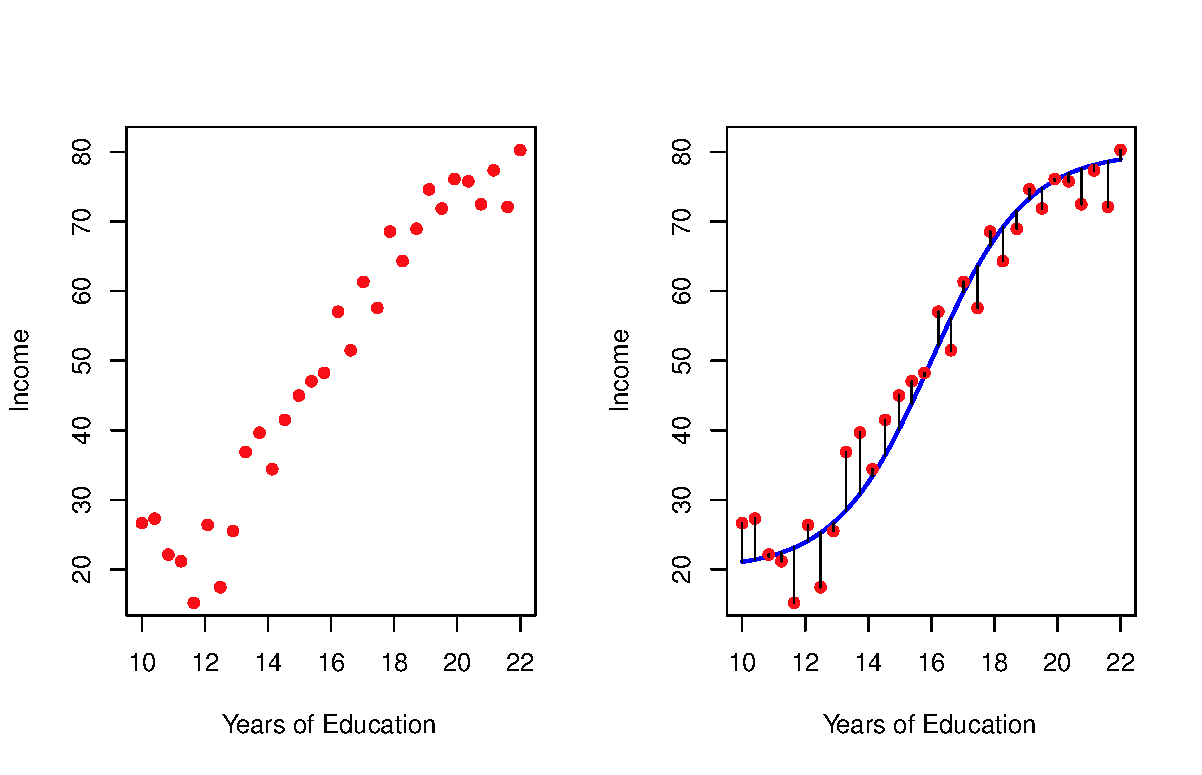
\includegraphics[width=0.92\textwidth,height=0.66\textheight,keepaspectratio]{2_2.pdf}
  \end{center}
  Income vs.\ years of education. The blue curve is the \emph{true}
  $f$ --- in real data we never see it.
  \islpsource{Figure 2.2}
\end{frame}

\begin{frame}{Reducible vs.\ irreducible error}
  Suppose we estimate $f$ by some $\hat{f}$ and predict
  $\hat{Y} = \hat{f}(X)$. Take expectation over a fixed $X$:
  \begin{block}{Decomposition}
    \[
      \boxed{\;
        E\bigl[(Y - \hat Y)^2 \mid X = x\bigr]
          = \underbrace{(f(x) - \hat f(x))^2}_{\text{reducible}}
           + \underbrace{\mathrm{Var}(\varepsilon)}_{\text{irreducible}}.
      \;}
    \]
  \end{block}
  \begin{takeaway}
    Better data and methods can shrink the reducible part to zero.
    No method, however clever, can reduce
    $\mathrm{Var}(\varepsilon)$.
  \end{takeaway}
\end{frame}

\begin{frame}{Why irreducible error exists}
  Even if we knew $f$ exactly, $\varepsilon$ may be non-zero because:
  \begin{readme}
    \begin{itemize}
      \item There are \emph{unmeasured} variables that affect $Y$
            (luck, family connections, mood --- not in our predictors).
      \item There are \emph{unmeasurable} variables (instrument
            noise, rounding, sampling).
      \item Even with all variables, $Y$ may be intrinsically
            stochastic.
    \end{itemize}
  \end{readme}
  \begin{takeaway}
    A model that achieves test MSE close to
    $\mathrm{Var}(\varepsilon)$ is essentially as good as it can get.
    We should not be disappointed that we cannot do better.
  \end{takeaway}
\end{frame}

\begin{frame}{Estimating $f$: from an unseen truth to a usable model}
  \begin{center}
  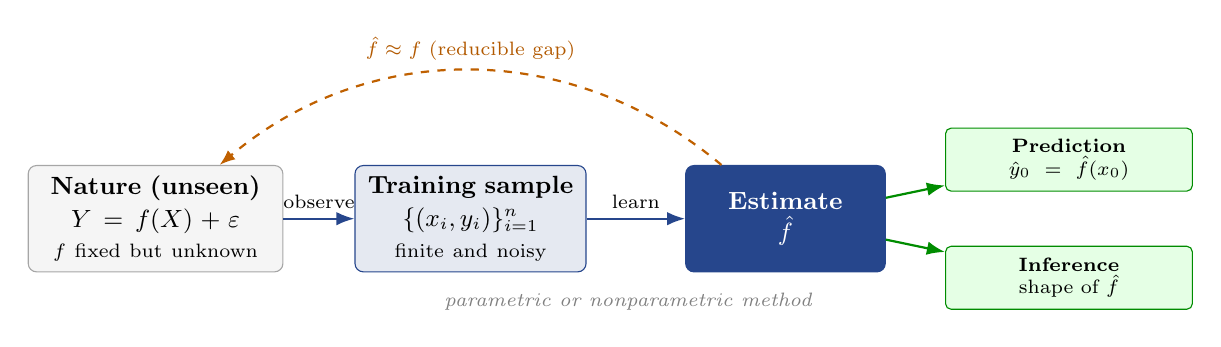
\begin{tikzpicture}[
    truth/.style={rounded corners=3pt,draw=gray!70,fill=gray!8,align=center,font=\small,text width=3.0cm,minimum height=1.35cm},
    data/.style={rounded corners=3pt,draw=accent,fill=accent!12,align=center,font=\small,text width=2.7cm,minimum height=1.35cm},
    est/.style={rounded corners=3pt,draw=accent,fill=accent,text=white,align=center,font=\small\bfseries,text width=2.3cm,minimum height=1.35cm},
    goal/.style={rounded corners=2pt,draw=green!55!black,fill=green!10,align=center,font=\scriptsize,text width=2.9cm,minimum height=0.8cm},
    arr/.style={-{Latex[length=2.3mm]},thick,draw=accent},
    cmp/.style={-{Latex[length=2mm]},thick,draw=orange!75!black,dashed}]
   \node[truth] (T) at (0,0) {\textbf{Nature (unseen)}\\[1pt]$Y=f(X)+\varepsilon$\\{\scriptsize $f$ fixed but unknown}};
   \node[data]  (D) at (4.0,0) {\textbf{Training sample}\\[1pt]$\{(x_i,y_i)\}_{i=1}^n$\\{\scriptsize finite and noisy}};
   \node[est]   (E) at (8.0,0) {Estimate\\$\hat f$};
   \draw[arr] (T)--(D) node[midway,above,font=\scriptsize,text=black]{observe};
   \draw[arr] (D)--(E) node[midway,above,font=\scriptsize,text=black]{learn};
   \node[font=\scriptsize\itshape,text=gray] at (6.0,-1.05){parametric or nonparametric method};
   \draw[cmp] (E) to[out=140,in=40] node[midway,above,font=\scriptsize,text=orange!70!black]{$\hat f\approx f$ (reducible gap)} (T);
   \node[goal] (g1) at (11.6,0.75){\textbf{Prediction}\\$\hat y_0=\hat f(x_0)$};
   \node[goal] (g2) at (11.6,-0.75){\textbf{Inference}\\shape of $\hat f$};
   \draw[arr,draw=green!55!black] (E)--(g1);
   \draw[arr,draw=green!55!black] (E)--(g2);
  \end{tikzpicture}
  \end{center}
  \begin{takeaway}We never see $f$ or $\varepsilon$ --- only a finite, noisy sample. A method turns that sample into $\hat f$; how close $\hat f$ lands to $f$ is the \emph{reducible} error, while $\varepsilon$ sets an \emph{irreducible} floor.\end{takeaway}
\end{frame}


% ============================================================
\section{Why f?}
% ============================================================

\begin{frame}{Two reasons to estimate $f$}
  In any application, you are doing one (or both) of:
  \begin{columns}[T]
    \begin{column}{0.48\textwidth}
      \begin{block}{Prediction}
        Given a new observation $X = x_0$, what value of $Y$ should we
        expect?
      \end{block}
    \end{column}
    \begin{column}{0.48\textwidth}
      \begin{block}{Inference}
        How does $Y$ depend on $X_1, \ldots, X_p$? Which predictors
        matter? Are the relationships linear?
      \end{block}
    \end{column}
  \end{columns}
  \begin{takeaway}
    Different goals favour different methods. A pure prediction
    problem often tolerates black-box models; an inference problem
    demands interpretability.
  \end{takeaway}
\end{frame}

\begin{frame}{Worked example: prediction goal}
  \begin{numexample}[Direct-mail marketing]
    A company has $X = $ (demographic features of a customer) and
    wants to predict $Y = $ likelihood the customer responds to a
    mailing.
    \begin{itemize}
      \item It does not matter \emph{why} a customer responds.
      \item Whatever model gives the best test-set accuracy wins.
      \item Random forests or neural networks are perfectly fine here.
    \end{itemize}
  \end{numexample}
\end{frame}

\begin{frame}{Worked example: inference goal}
  \begin{numexample}[Wage data]
    Researchers want to estimate the \emph{return to education}: how
    much does an extra year of education raise wages, holding all
    else equal?
    \begin{itemize}
      \item A black-box prediction is useless --- we need a coefficient.
      \item A linear-regression coefficient (with a confidence
            interval) answers the question directly.
      \item Random forests would predict accurately but tell us
            nothing about the magnitude of effects.
    \end{itemize}
  \end{numexample}
\end{frame}


% ============================================================
\section{Estimating}
% ============================================================

\begin{frame}{Two strategies to estimate $f$}
  \begin{columns}[T]
    \begin{column}{0.48\textwidth}
      \begin{block}{Parametric}
        Assume $f$ has a particular functional form (e.g.\ linear)
        governed by a finite set of parameters $\theta$. Estimate
        $\theta$ from data.
      \end{block}
    \end{column}
    \begin{column}{0.48\textwidth}
      \begin{block}{Nonparametric}
        Make no global assumption about the form of $f$. Let the
        data determine $f$ as flexibly as possible.
      \end{block}
    \end{column}
  \end{columns}
  \begin{takeaway}
    These two strategies trade off bias against variance and
    interpretability against flexibility.
  \end{takeaway}
\end{frame}

\begin{frame}{Parametric vs.\ nonparametric: a one-predictor illustration}
  \begin{center}
    
\includegraphics[width=0.9\textwidth,height=0.56\textheight,keepaspectratio]{ch02_param_vs_nonparam.png}
  \end{center}
  \begin{takeaway}The straight line (two parameters) \emph{underfits} the curvature --- misspecification bias. The kernel smoother assumes no fixed form and tracks $f$ closely. Flexibility buys lower bias, at the cost of higher variance.\end{takeaway}
\end{frame}

\begin{frame}{The parametric approach: two-step recipe}
  \begin{block}{Recipe}
    \begin{enumerate}
      \item Choose a functional form. For example, the linear form
            $f(X) = \beta_0 + \beta_1 X_1 + \cdots + \beta_p X_p$.
      \item Fit the model. Use a procedure (e.g.\ ordinary least
            squares) to estimate $\beta_0, \ldots, \beta_p$.
    \end{enumerate}
  \end{block}
  \begin{readme}
    This reduces estimating an infinite-dimensional function to
    estimating $p + 1$ numbers.
  \end{readme}
\end{frame}

\begin{frame}{Linear fit on Income}
  \begin{center}
    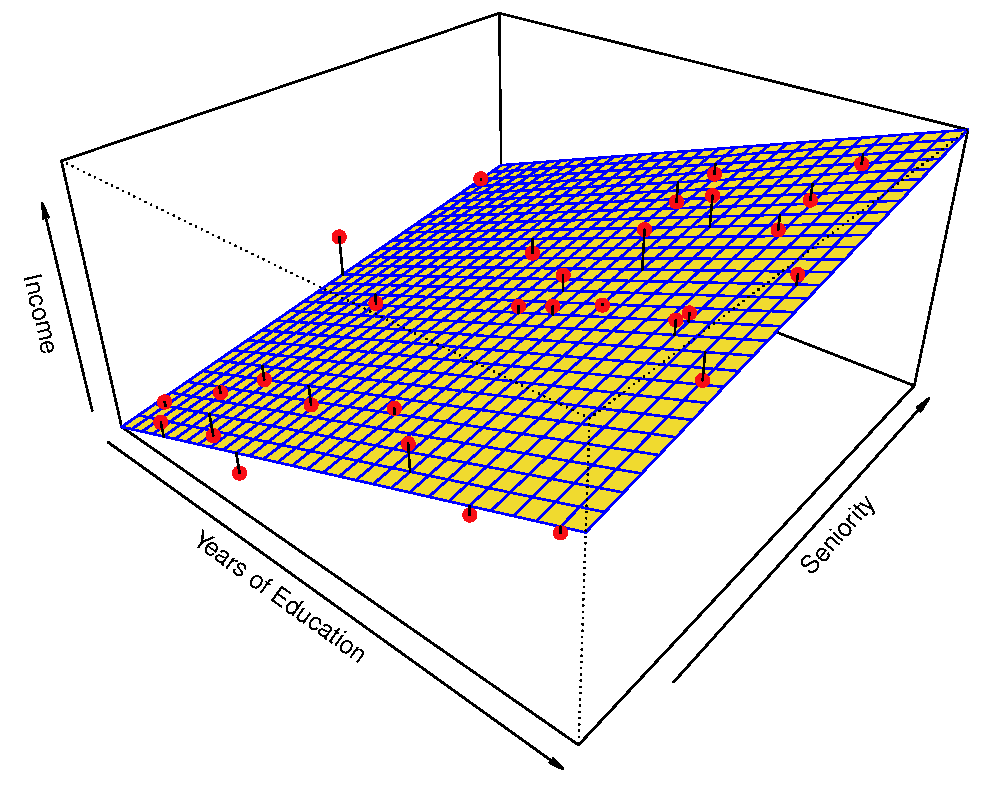
\includegraphics[width=0.85\textwidth,height=0.66\textheight,keepaspectratio]{2_4.pdf}
  \end{center}
  The yellow plane is the linear regression estimate. It captures the
  main increasing trends but misses the curvature --- this is
  \emph{bias} from a misspecified functional form.
  \islpsource{Figure 2.4}
\end{frame}

\begin{frame}{Pros and cons of parametric methods}
  \begin{columns}[T]
    \begin{column}{0.48\textwidth}
      \textbf{Pros}
      \begin{itemize}
        \item Few parameters $\Rightarrow$ low variance.
        \item Interpretable: parameters \emph{are} the model.
        \item Inference (SEs, $p$-values) well-developed.
        \item Computationally cheap.
      \end{itemize}
    \end{column}
    \begin{column}{0.48\textwidth}
      \textbf{Cons}
      \begin{itemize}
        \item Bias if the true $f$ is not in the assumed family.
        \item Sensitive to outliers when the form is wrong.
        \item Cannot capture interactions unless explicitly added.
      \end{itemize}
    \end{column}
  \end{columns}
\end{frame}

\begin{frame}{Nonparametric Income fit (smooth thin-plate spline)}
  \begin{center}
    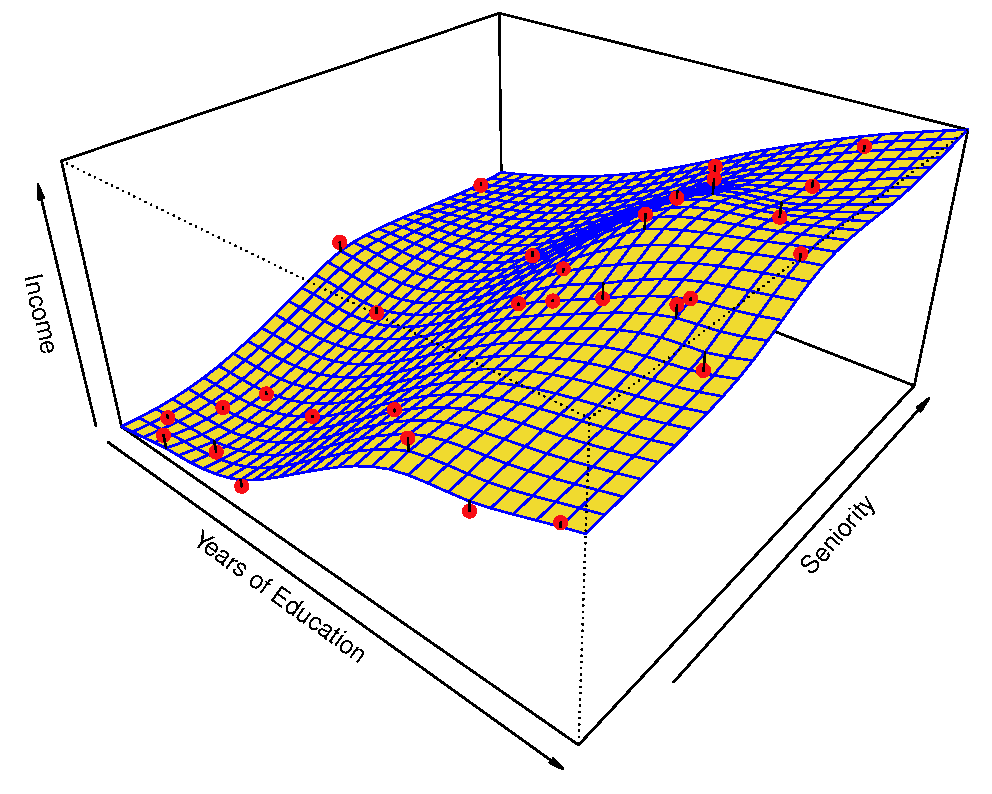
\includegraphics[width=0.85\textwidth,height=0.66\textheight,keepaspectratio]{2_5.pdf}
  \end{center}
  The yellow surface is now curved, matching the true $f$ much more
  closely. No misspecification bias --- this is what you want when you
  do not know the functional form.
  \islpsource{Figure 2.5}
\end{frame}

\begin{frame}{Nonparametric Income fit (rough thin-plate spline)}
  \begin{center}
    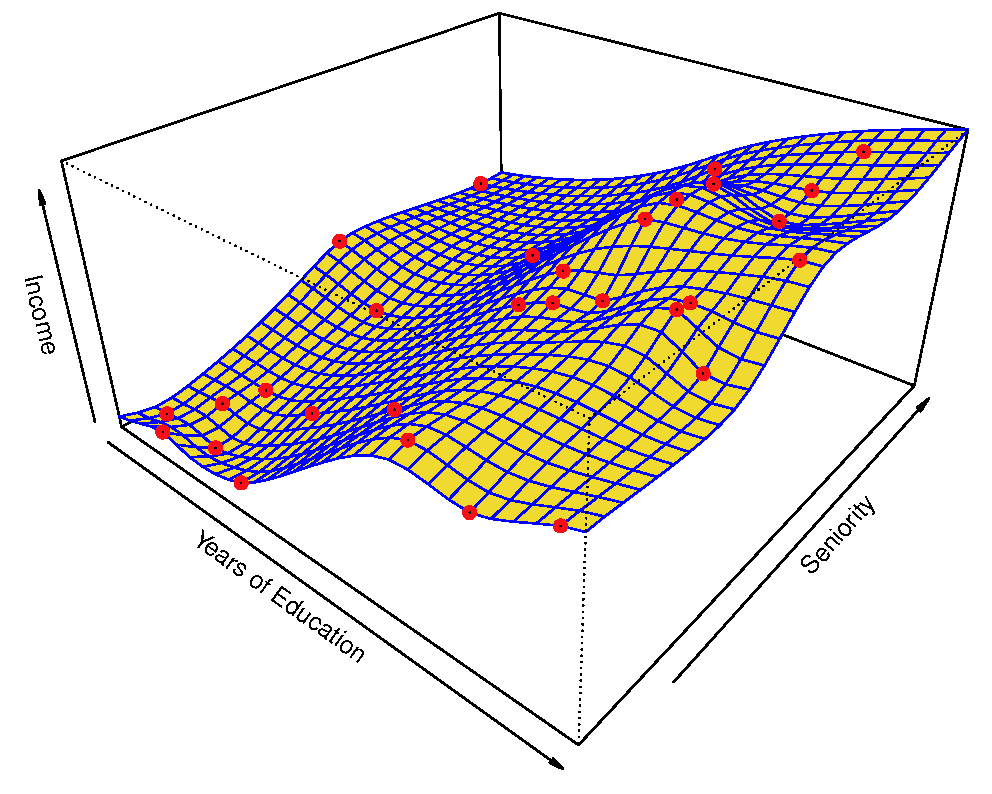
\includegraphics[width=0.85\textwidth,height=0.66\textheight,keepaspectratio]{2_6.pdf}
  \end{center}
  This surface passes through nearly every training point --- training
  error is essentially zero. But the bumps respond to \emph{noise},
  not signal. Classical \emph{overfitting}.
  \islpsource{Figure 2.6}
\end{frame}


\begin{frame}{Exercise 2.1 --- Parametric vs.\ Nonparametric [Concept]}
\begin{exercise}
\begin{enumerate}
  \item Define, in one sentence each, a \emph{parametric} and a
        \emph{nonparametric} method.
  \item For each, does the number of parameters stay fixed in advance
        or grow with the sample size $n$?
  \item Classify: (i) OLS linear regression, (ii) KNN,
        (iii) a fixed cubic polynomial regression,
        (iv) a thin-plate spline whose smoothing is chosen by
        cross-validation.
  \item You have $n=40$, $p=1$; the scatter is clearly curved but you
        do not know its form. Which family would you choose, and what
        is the main risk of the \emph{other} family here?
\end{enumerate}
\end{exercise}
\end{frame}

\begin{frame}{Solution --- Exercise 2.1 (1/2)}
\begin{solutionbox}
\begin{enumerate}
  \item \textbf{Parametric:} assume a fixed functional form for $f$
        governed by a finite parameter vector $\theta$, then estimate
        $\theta$. \textbf{Nonparametric:} make no global assumption
        about the form of $f$; let the data determine it, seeking a
        fit close to the points without being too rough.
  \item Parametric: the number of parameters is \emph{fixed in
        advance} (does not grow with $n$) --- the family is chosen
        before seeing the data, so extra observations only pin down
        the same few components of $\theta$ more precisely.
        Nonparametric: effective complexity \emph{grows with} $n$ ---
        with more data the fit is allowed to wiggle in more places
        (think of KNN, where every new training point can reshape the
        prediction in its neighbourhood).
\end{enumerate}
\end{solutionbox}
\end{frame}

\begin{frame}{Solution --- Exercise 2.1 (2/2)}
\begin{solutionbox}
\begin{enumerate}\setcounter{enumi}{2}
  \item (i) OLS linear regression: \textbf{parametric} --- the form
        $\beta_0+\beta_1X_1+\cdots+\beta_pX_p$ is fixed, and fitting
        only estimates $p+1$ numbers.
        (ii) KNN: \textbf{nonparametric} --- no formula for $f$ is
        written down; the prediction is a local vote that adapts to
        wherever the data lie.
        (iii) Fixed cubic polynomial: \textbf{parametric} --- curved,
        but still a fixed form with four coefficients
        $\beta_0,\ldots,\beta_3$ chosen in advance.
        (iv) Thin-plate spline with CV-chosen smoothing:
        \textbf{nonparametric} --- no fixed global form; the data,
        via cross-validation, determine the effective flexibility.
  \item Prefer \textbf{nonparametric} (flexible), because a fixed form
        is unknown and a parametric guess risks large
        \emph{bias from misspecification}. Caveat: with only $n=40$ a
        very flexible fit risks high \emph{variance}/overfitting --- so
        pick the smoothing by cross-validation.
\end{enumerate}
\smallskip
{\itshape Common mistake: equating ``nonlinear'' with
``nonparametric''. A cubic polynomial is curved yet fully parametric
--- what matters is whether the form and its parameter count are fixed
before seeing the data.}
\end{solutionbox}
\end{frame}


% ============================================================
\section{Flexibility}
% ============================================================

\begin{frame}{The flexibility-interpretability trade-off}
  Methods can be ranked along a flexibility spectrum:
  \begin{center}
  \footnotesize
  \begin{tabular}{lcc}
    \toprule
    \textbf{Method} & \textbf{Flexibility} & \textbf{Interpretability} \\
    \midrule
    Subset selection / Lasso & low & high \\
    Linear regression & low & high \\
    GAMs / splines & medium & medium \\
    Trees & medium & medium \\
    Bagging / random forests & high & low \\
    Boosting & high & low \\
    Deep learning & very high & very low \\
    \bottomrule
  \end{tabular}
  \end{center}
  \begin{takeaway}Reading top to bottom, flexibility rises while interpretability falls --- the two trade off. Choose the \emph{least} flexible method that still captures the signal.\end{takeaway}
\end{frame}

\begin{frame}{The trade-off as a map: where each method sits}
  \begin{center}
  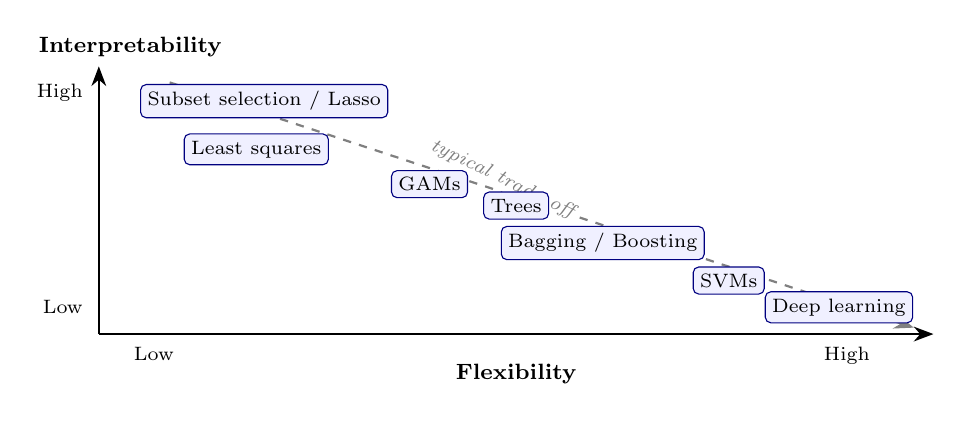
\begin{tikzpicture}[xscale=1.0,yscale=0.68,
      meth/.style={draw=blue!50!black,fill=blue!6,rounded corners=2pt,
                   inner sep=2.5pt,font=\scriptsize}]
    % axes
    \draw[-{Stealth[length=2.5mm]},thick] (0,0) -- (10.6,0);
    \node[font=\footnotesize\bfseries] at (5.3,-0.75) {Flexibility};
    \draw[-{Stealth[length=2.5mm]},thick] (0,0) -- (0,5.0);
    \node[above,font=\footnotesize\bfseries] at (0.4,5.0) {Interpretability};
    \node[below,font=\scriptsize] at (0.7,-0.06) {Low};
    \node[below,font=\scriptsize] at (9.5,-0.06) {High};
    \node[left,font=\scriptsize] at (-0.08,4.5) {High};
    \node[left,font=\scriptsize] at (-0.08,0.5) {Low};
    % typical trade-off diagonal
    \draw[dashed,gray,-{Stealth[length=2.5mm]},thick]
          (0.9,4.70) -- (10.35,0.12)
          node[pos=0.44,above,sloped,font=\scriptsize\itshape,
               fill=white,inner sep=1pt]{typical trade-off};
    % methods (high interpretability / low flexibility -> the reverse)
    \node[meth] at (2.10,4.35) {Subset selection / Lasso};
    \node[meth] at (2.00,3.45) {Least squares};
    \node[meth] at (4.20,2.80) {GAMs};
    \node[meth] at (5.30,2.40) {Trees};
    \node[meth] at (6.40,1.70) {Bagging / Boosting};
    \node[meth] at (8.00,1.00) {SVMs};
    \node[meth] at (9.40,0.50) {Deep learning};
  \end{tikzpicture}
  \end{center}
  \begin{takeaway}Every method buys flexibility by selling interpretability --- there is no upper-right corner. Inference pulls you up-left; pure prediction slides you down the diagonal.\end{takeaway}
\end{frame}

\begin{frame}{Why ever choose a less-flexible method?}
  Several good reasons:
  \begin{takeaway}
    \begin{itemize}
      \item \textbf{Inference.} Coefficients of a linear regression
            have meaning; weights of a neural network usually don't.
      \item \textbf{Sample size.} With $n$ small, flexible methods
            overfit.
      \item \textbf{Stability.} Simple models change little as the
            data change a little.
      \item \textbf{Communication.} A non-technical audience will not
            accept a black box.
      \item \textbf{Regulation.} Credit, health, and insurance often
            require interpretability by law.
    \end{itemize}
  \end{takeaway}
\end{frame}


\begin{frame}{Exercise 2.2 --- Flexibility vs.\ Interpretability [Concept]}
\begin{exercise}
\begin{enumerate}
  \item Rank these by flexibility, low to high: linear regression,
        deep neural network, lasso, random forest, GAM/spline.
  \item Give \emph{two} distinct reasons to deliberately pick a
        \emph{less}-flexible method even if a flexible one predicts a
        little better.
  \item True or false, with reason: ``More flexible always means
        lower test error.''
  \item A credit-scoring model must, by regulation, explain every
        decision. Which end of the spectrum, and name one suitable
        method.
\end{enumerate}
\end{exercise}
\end{frame}

\begin{frame}{Solution --- Exercise 2.2 (1/2)}
\begin{solutionbox}
\begin{enumerate}
  \item lasso $\approx$ linear regression (low) $<$ GAM/spline
        (medium) $<$ random forest (high) $<$ deep neural network
        (very high). Why this order: the lasso is a
        \emph{constrained} linear model, so it can be at most as
        flexible as unpenalised least squares; a GAM/spline relaxes
        linearity to a smooth curve per predictor; a random forest
        adds interactions and abrupt jumps; a deep network can
        approximate essentially any function.
  \item Any two of: \emph{inference} (coefficients carry meaning);
        \emph{small $n$} (flexible methods overfit); \emph{stability}
        (simple models change little when the data change a little);
        \emph{communication} to a non-technical audience;
        \emph{regulation}/legal requirements. Each reason deliberately
        trades a little predictive accuracy for something the
        application values more.
\end{enumerate}
\end{solutionbox}
\end{frame}

\begin{frame}{Solution --- Exercise 2.2 (2/2)}
\begin{solutionbox}
\begin{enumerate}\setcounter{enumi}{2}
  \item \textbf{False.} Test error is U-shaped in flexibility: past
        the optimum, variance grows faster than bias falls, so test
        error \emph{rises} (overfitting). Extra flexibility helps only
        while systematic signal remains to be captured; beyond that
        point the model starts fitting noise. Only \emph{training}
        error always falls as flexibility grows.
  \item The \textbf{low-flexibility, interpretable} end --- e.g.\ a
        (penalised) logistic/linear regression or a small decision
        tree, whose decisions can be read off directly. Coefficients
        (or a short path of splits) provide the per-case justification
        the regulation demands.
\end{enumerate}
\smallskip
{\itshape Common mistake: reading the flexibility ranking in part 1 as
a quality ranking. The U-shaped test error means the best method
depends on the data and the goal --- ``more flexible'' is not
``better'' by default.}
\end{solutionbox}
\end{frame}


% ============================================================
\section{Supervision}
% ============================================================

\begin{frame}{Supervised vs.\ unsupervised learning}
  \begin{columns}[T]
    \begin{column}{0.48\textwidth}
      \begin{block}{Supervised}
        For each observation $i = 1, \ldots, n$ we have predictors
        $x_i$ and a corresponding response $y_i$.
      \end{block}
      Goal: learn the map $X \mapsto Y$.
    \end{column}
    \begin{column}{0.48\textwidth}
      \begin{block}{Unsupervised}
        For each observation we have only $x_i$, no response $y_i$.
      \end{block}
      Goal: discover structure in $X$.
    \end{column}
  \end{columns}
  \begin{takeaway}
    Most of this course focuses on supervised learning. Chapter 12
    returns to the unsupervised case.
  \end{takeaway}
\end{frame}


% ============================================================
\section{Reg vs Class}
% ============================================================

\begin{frame}{Regression vs.\ classification}
  The type of $Y$ determines the problem type:
  \begin{readme}
    \begin{itemize}
      \item Quantitative $Y$ $\Rightarrow$ \emph{regression problem}.
      \item Qualitative $Y$ $\Rightarrow$ \emph{classification
            problem}.
    \end{itemize}
  \end{readme}
  \begin{alertblock}{Common confusion}
    Whether you have a regression or a classification problem depends
    on $Y$, \emph{not} on the $X_j$. A categorical predictor in a
    regression on a numeric response is still a regression.
  \end{alertblock}
\end{frame}


% ============================================================
\section{Accuracy}
% ============================================================

\begin{frame}{Mean squared error: the central regression metric}
  \begin{block}{Definition}
    \[
      \boxed{\;
        \mathrm{MSE} = \frac{1}{n}\sum_{i=1}^n
          \bigl(y_i - \hat f(x_i)\bigr)^2.
      \;}
    \]
  \end{block}
  \begin{readme}[Reading the formula]
    $y_i-\hat f(x_i)$ is the \emph{residual} for point $i$ (truth minus
    prediction); square it so over- and under-shoots both count and big
    misses hurt more; then average over all $n$ points. Squaring makes
    MSE convex and differentiable --- friendly to optimisation --- and
    ties it historically to Gaussian errors.
  \end{readme}
\end{frame}

\begin{frame}{Training MSE vs.\ test MSE}
  \begin{columns}[T]
    \begin{column}{0.48\textwidth}
      \begin{block}{Training MSE}
        MSE on the data used to fit the model. Always
        \emph{over-optimistic} --- the model has been bent to fit
        these points.
      \end{block}
    \end{column}
    \begin{column}{0.48\textwidth}
      \begin{block}{Test MSE}
        MSE on \emph{new}, held-out observations. The honest measure
        of predictive performance.
      \end{block}
    \end{column}
  \end{columns}
  \begin{alertblock}{The cardinal sin}
    Training MSE is essentially never what we care about. We minimise
    training MSE in order to make test MSE small --- not as a goal in
    itself.
  \end{alertblock}
\end{frame}

\begin{frame}{Simulated data: candidate fits and their train/test MSE}
  \begin{center}
    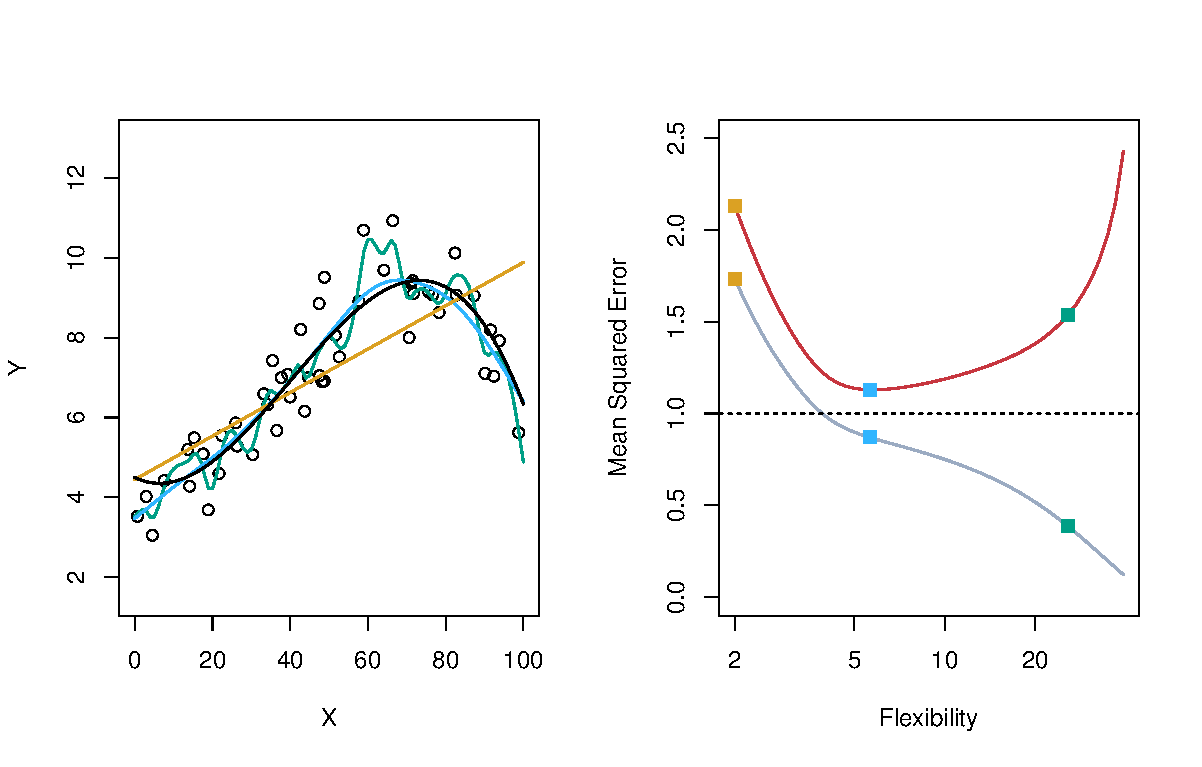
\includegraphics[width=0.95\textwidth,height=0.66\textheight,keepaspectratio]{2_9.pdf}
  \end{center}
  \islpsource{Figure 2.9}
\end{frame}

\begin{frame}{Reading the simulation}
  \begin{readme}
    Left: simulated data (black dots), the true $f$ (black), and
    three fits: linear (orange), moderate spline (blue), and very
    flexible spline (green).\\
    Right: training MSE (grey) and test MSE (red) as a function of
    flexibility.
  \end{readme}
  \begin{takeaway}[Three observations]
    \begin{itemize}
      \item Training MSE \emph{always} decreases as flexibility grows.
      \item Test MSE has a U-shape: first decreases, then increases.
      \item The optimum is where the U bottoms out --- which we cannot
            read off the training MSE.
    \end{itemize}
  \end{takeaway}
\end{frame}

\begin{frame}{Simulating the U-shape: training vs. test MSE}
  \begin{center}
    
\includegraphics[width=0.9\textwidth,height=0.58\textheight,keepaspectratio]{ch02_flexibility_mse.png}
  \end{center}
  \begin{takeaway}Fitting polynomials of growing degree: training MSE falls monotonically while test MSE is U-shaped, minimised at moderate flexibility.\end{takeaway}
\end{frame}


\begin{frame}{Exercise 2.3 --- Why Training MSE Understates Test MSE [Concept]}
\begin{exercise}
\begin{enumerate}
  \item Explain in words why, for the same model, training MSE is
        almost always \emph{smaller} than test MSE.
  \item As flexibility increases, describe the behaviour of
        (i) training MSE and (ii) test MSE.
  \item A student fits a degree-15 polynomial to 20 points and gets
        training MSE $\approx 0$, concluding the model is excellent.
        What is wrong, and what should they report instead?
  \item Define \emph{overfitting} in one sentence, in terms of
        training vs.\ test error.
\end{enumerate}
\end{exercise}
\end{frame}

\begin{frame}{Solution --- Exercise 2.3 (1/2)}
\begin{solutionbox}
\begin{enumerate}
  \item The parameters are chosen to \emph{minimise error on the
        training data}, so the fit adapts to that sample's specific
        noise. New observations carry different noise the model has
        never seen, so error on them is larger. Training error is
        therefore an \emph{optimistically biased} estimate of test
        error --- the model is graded on the very questions it was
        tuned to answer.
  \item (i) Training MSE decreases \emph{monotonically} as flexibility
        grows: a more flexible family contains the less flexible fits,
        so it can only match the training points at least as well.
        (ii) Test MSE is \emph{U-shaped}: it falls while added
        flexibility captures genuine signal (bias shrinks), reaches a
        minimum, then rises once the model starts chasing noise
        (variance takes over).
\end{enumerate}
\end{solutionbox}
\end{frame}

\begin{frame}{Solution --- Exercise 2.3 (2/2)}
\begin{solutionbox}
\begin{enumerate}\setcounter{enumi}{2}
  \item Near-zero training error only means the flexible polynomial
        \emph{interpolates} the 20 points, noise included --- a
        degree-15 polynomial has 16 coefficients, nearly one per
        observation, so it can pass through almost every point by
        construction. That says nothing about new data. They should
        report \textbf{test MSE} on held-out data (or a
        cross-validated error), which would very likely be far larger
        than the training MSE.
  \item \textbf{Overfitting:} when a model has low training error but
        high test error because it has fit noise rather than signal.
\end{enumerate}
\smallskip
{\itshape Common mistake: treating zero training error as proof that
the model has ``learned the data''. It has \emph{memorised} them ---
interpolation is not generalisation, and only performance on unseen
data counts.}
\end{solutionbox}
\end{frame}


% ============================================================
\section{Bias-Variance}
% ============================================================

\begin{frame}{The bias-variance decomposition}
  Fix a test point $x_0$ and average over training sets:
  \begin{block}{Decomposition}
    \[
      \boxed{\;
        E\bigl[(y_0 - \hat f(x_0))^2\bigr]
          = \mathrm{Var}(\hat f(x_0))
          + \bigl[\mathrm{Bias}(\hat f(x_0))\bigr]^2
          + \mathrm{Var}(\varepsilon).
      \;}
    \]
  \end{block}
\end{frame}

\begin{frame}{Reading the three pieces}
  \begin{readme}
    \begin{tabular}{@{}cl@{}}
      \toprule
      \textbf{Piece} & \textbf{Meaning} \\
      \midrule
      $\mathrm{Var}(\hat f(x_0))$ &
        Variability of the estimate across training sets \\
      $\mathrm{Bias}(\hat f(x_0)) = E[\hat f(x_0)] - f(x_0)$ &
        Systematic error from a too-simple model \\
      $\mathrm{Var}(\varepsilon) = \sigma^2$ &
        Irreducible noise (the floor) \\
      \bottomrule
    \end{tabular}
  \end{readme}
  \begin{takeaway}
    Every prediction error has these three sources. The art of
    statistical learning is balancing the first two.
  \end{takeaway}
\end{frame}

\begin{frame}{What is bias?}
  \begin{block}{Definition}
    Bias is the error introduced by approximating a complicated
    reality by a simpler model.
  \end{block}
  \begin{numexample}
    A linear model has high bias if the truth is curved. A constant
    model (predicting the global mean) has very high bias unless $Y$
    is essentially flat in $X$.
  \end{numexample}
  \begin{takeaway}
    Bias \emph{decreases} as a method becomes more flexible.
  \end{takeaway}
\end{frame}

\begin{frame}{What is variance?}
  \begin{block}{Definition}
    Variance is how much $\hat f$ would change if we re-fit it on a
    different training set drawn from the same distribution.
  \end{block}
  \begin{numexample}
    A flexible method bends to whatever data it sees, so two training
    sets give very different fits. A linear model is much more
    stable.
  \end{numexample}
  \begin{takeaway}
    Variance \emph{increases} as a method becomes more flexible.
  \end{takeaway}
\end{frame}

\begin{frame}{Bias and variance trade off}
  As we increase flexibility:
  \begin{itemize}
    \item Bias goes \emph{down}.
    \item Variance goes \emph{up}.
    \item Their sum is a U-shape: the bias-variance trade-off.
    \item The optimal model lies at the bottom of the U.
  \end{itemize}
\end{frame}

\begin{frame}{The bias-variance trade-off, schematically}
  \begin{center}
  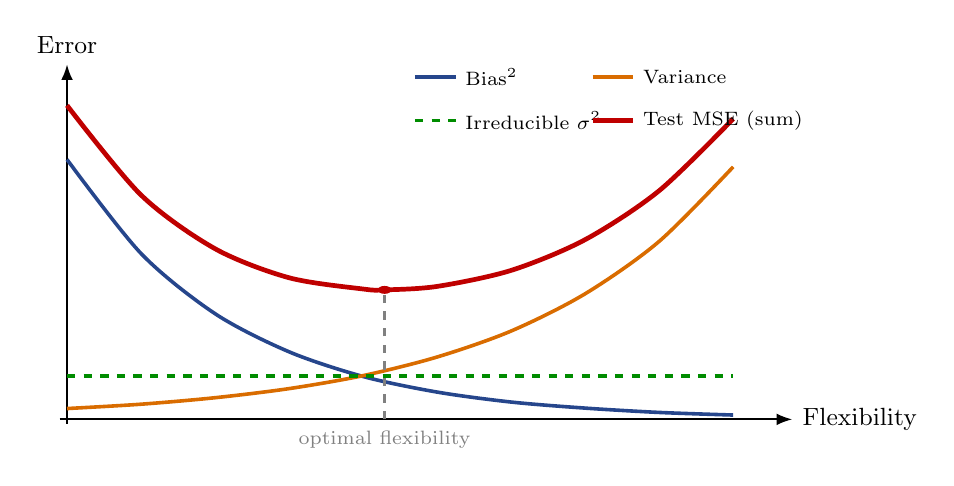
\begin{tikzpicture}[xscale=0.94,yscale=0.55]
   \draw[-{Latex[length=2mm]},thick] (-0.1,0) -- (9.8,0) node[right,font=\small]{Flexibility};
   \draw[-{Latex[length=2mm]},thick] (0,-0.1) -- (0,8.2) node[above,font=\small]{Error};
   \draw[draw=accent,line width=1.3pt] plot[smooth] coordinates {(0,6.00)(1,3.83)(2,2.44)(3,1.56)(4,0.99)(5,0.63)(6,0.40)(7,0.26)(8,0.16)(9,0.10)};
   \draw[draw=orange!85!black,line width=1.3pt] plot[smooth] coordinates {(0,0.25)(1,0.35)(2,0.50)(3,0.71)(4,1.01)(5,1.44)(6,2.04)(7,2.90)(8,4.11)(9,5.83)};
   \draw[draw=green!55!black,line width=1.2pt,dashed] (0,1.0)--(9,1.0);
   \draw[draw=red!75!black,line width=1.7pt] plot[smooth] coordinates {(0,7.25)(1,5.18)(2,3.94)(3,3.27)(4,3.01)(4.29,2.99)(5,3.07)(6,3.44)(7,4.15)(8,5.28)(9,6.94)};
   \draw[gray,dashed,line width=1pt] (4.29,0)--(4.29,2.99);
   \fill[red!75!black] (4.29,2.99) circle (2.6pt);
   \node[font=\scriptsize,text=gray,below] at (4.29,-0.05) {optimal flexibility};
   \begin{scope}[shift={(4.7,7.9)}]
     \draw[draw=accent,line width=1.3pt] (0,0)--(0.55,0); \node[right,font=\scriptsize] at (0.55,0){Bias$^2$};
     \draw[draw=orange!85!black,line width=1.3pt] (2.4,0)--(2.95,0); \node[right,font=\scriptsize] at (2.95,0){Variance};
     \draw[draw=green!55!black,line width=1.2pt,dashed] (0,-1.0)--(0.55,-1.0); \node[right,font=\scriptsize] at (0.55,-1.0){Irreducible $\sigma^2$};
     \draw[draw=red!75!black,line width=1.7pt] (2.4,-1.0)--(2.95,-1.0); \node[right,font=\scriptsize] at (2.95,-1.0){Test MSE (sum)};
   \end{scope}
  \end{tikzpicture}
  \end{center}
  \begin{takeaway}Test MSE $=$ bias$^2 +$ variance $+ \sigma^2$; it bottoms out where falling bias meets rising variance.\end{takeaway}
\end{frame}

\begin{frame}{Bias, variance, and test MSE across flexibility}
  \begin{center}
    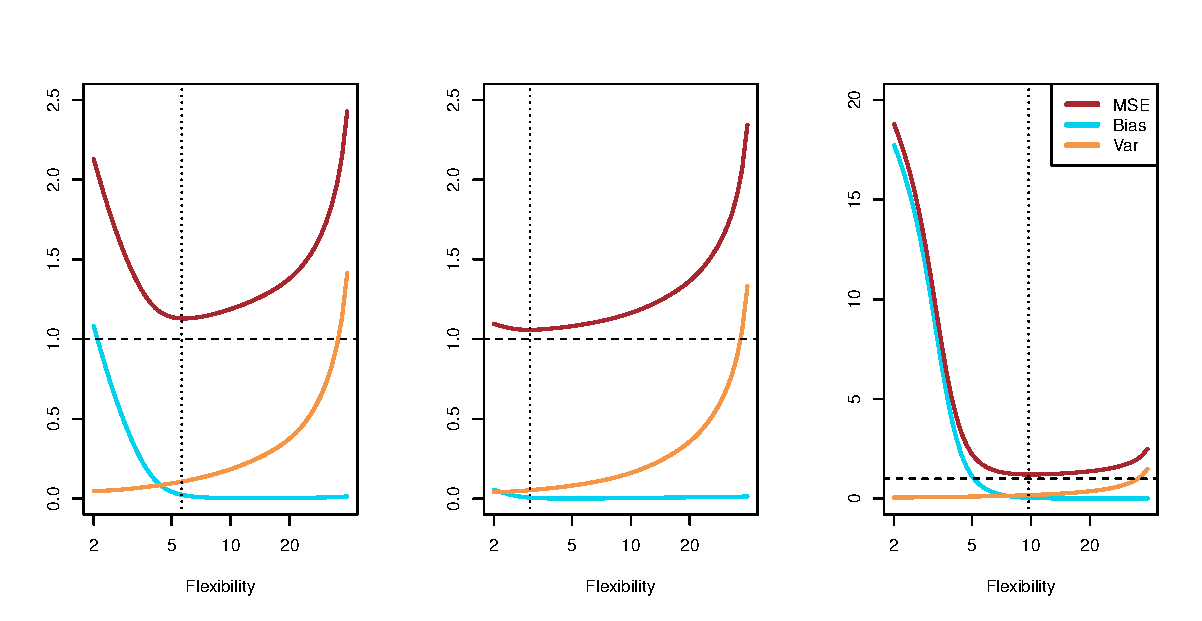
\includegraphics[width=0.95\textwidth,height=0.66\textheight,keepaspectratio]{2_12.pdf}
  \end{center}
  Solid blue: bias squared. Solid orange: variance. Solid red: test
  MSE = bias$^2$ + variance + $\sigma^2$. Vertical dashed line: the
  flexibility level that minimises test MSE.
  \islpsource{Figure 2.12}
\end{frame}


\begin{frame}{Mini-check: bias and variance}
  \begin{readme}[Match each statement to bias or variance]
    \begin{enumerate}
      \item ``A linear model on a curved truth.'' \hfill (\,?\,)
      \item ``A KNN classifier with $K = 1$.''      \hfill (\,?\,)
      \item ``Refitting on a different training sample changes the
            answer a lot.'' \hfill (\,?\,)
      \item ``The model is too simple to capture the relationship.''
            \hfill (\,?\,)
    \end{enumerate}
  \end{readme}
  \begin{takeaway}[Answers]
    1.\ high bias.\quad 2.\ high variance.\quad 3.\ high variance.\quad
    4.\ high bias.
  \end{takeaway}
\end{frame}

\begin{frame}{Exercise 2.4 --- Bias-Variance Decomposition (numbers) [Math]}
\begin{exercise}
The expected test MSE at a point $x_0$ decomposes as
\[
  E\bigl[(y_0-\hat f(x_0))^2\bigr]
   = \mathrm{Var}(\hat f(x_0)) + \bigl[\mathrm{Bias}(\hat f(x_0))\bigr]^2
   + \mathrm{Var}(\varepsilon).
\]
\begin{enumerate}
  \item Which term(s) are reducible and which is irreducible?
  \item At $x_0$: over many training sets $E[\hat f(x_0)]=9.0$ while
        the truth $f(x_0)=10.0$; $\mathrm{Var}(\hat f(x_0))=1.5$;
        $\sigma^2=\mathrm{Var}(\varepsilon)=2.0$. Compute the bias,
        the squared bias, and the expected test MSE.
  \item A more flexible method has $\mathrm{Var}(\hat f)=4.0$ and
        $\mathrm{Bias}=-0.2$ at $x_0$. Which method wins at $x_0$?
  \item What is the smallest possible expected test MSE at $x_0$, and
        why?
\end{enumerate}
\end{exercise}
\end{frame}

\begin{frame}{Solution --- Exercise 2.4 (1/2)}
\begin{solutionbox}
\begin{enumerate}
  \item $\mathrm{Var}(\hat f)$ and $\mathrm{Bias}^2$ are
        \textbf{reducible}: both depend on the estimator $\hat f$, so
        a better method, more data, or better-tuned flexibility can
        shrink them. $\mathrm{Var}(\varepsilon)=\sigma^2$ is
        \textbf{irreducible}: it is a property of the data-generating
        process itself, and no choice of $\hat f$ can touch it.
  \item The decomposition applies term by term, so we substitute the
        given quantities. First the bias, from its definition:
        \[
          \mathrm{Bias}=E[\hat f]-f=9.0-10.0=-1.0,
          \qquad \mathrm{Bias}^2=(-1.0)^2=1.0.
        \]
        Then the expected test MSE is the sum of the three pieces:
        \[
          \text{MSE}=\underbrace{1.5}_{\text{Var}}
          +\underbrace{1.0}_{\text{Bias}^2}
          +\underbrace{2.0}_{\sigma^2}=4.5.
        \]
        Interpretation: almost half of the total ($2.0$ of $4.5$) is
        noise that no model could ever remove.
\end{enumerate}
\end{solutionbox}
\end{frame}

\begin{frame}{Solution --- Exercise 2.4 (2/2)}
\begin{solutionbox}
\begin{enumerate}\setcounter{enumi}{2}
  \item Same recipe for the flexible method:
        $\mathrm{Bias}^2=(-0.2)^2=0.04$, so
        MSE $=4.0+0.04+2.0=6.04$. Since $4.5<6.04$, the
        \emph{less}-flexible method (Ex.\ part 2) wins here: its lower
        variance more than offsets its larger bias. In numbers,
        flexibility cut the squared bias by $0.96$ (from $1.00$ to
        $0.04$) but raised the variance by $2.5$ (from $1.5$ to
        $4.0$) --- a bad trade at this $x_0$.
  \item The floor is $\sigma^2=2.0$, reached only if both variance and
        squared bias are zero. No method can beat the irreducible
        noise $\mathrm{Var}(\varepsilon)$: even the true $f$, known
        exactly, would still miss new observations by their noise.
\end{enumerate}
\smallskip
{\itshape Common mistake: forgetting to square the bias (adding $-1.0$
or $-0.2$ directly), or expecting a negative bias to \emph{lower} the
MSE. Only $\mathrm{Bias}^2$ enters, so the sign is irrelevant ---
systematic over- and under-prediction hurt equally.}
\end{solutionbox}
\end{frame}

\begin{frame}{Exercise 2.5 --- Reading the U-shaped Test-Error Curve [Concept]}
\begin{exercise}
A plot has flexibility on the $x$-axis and error on the $y$-axis. It
shows a monotonically decreasing curve, a U-shaped curve, and a
horizontal dashed line at the bottom.
\begin{enumerate}
  \item Which curve is training error, which is test error, and what
        does the dashed line represent?
  \item Label the regions left and right of the U's minimum as
        underfitting or overfitting, and say whether bias or variance
        dominates in each.
  \item Why can the optimal flexibility \emph{not} be found from the
        training-error curve alone?
  \item In practice, how do we locate the test-error minimum without a
        large held-out set?
\end{enumerate}
\end{exercise}
\end{frame}

\begin{frame}{Solution --- Exercise 2.5 (1/2)}
\begin{solutionbox}
\begin{enumerate}
  \item Monotonically decreasing $=$ \textbf{training error}: extra
        flexibility always lets the model fit the training points at
        least as well. U-shaped $=$ \textbf{test error}: it improves
        while genuine signal is being captured, then worsens. Dashed
        line $=$ \textbf{irreducible error}
        $\mathrm{Var}(\varepsilon)=\sigma^2$ --- the noise floor that
        expected test error can approach but never fall below.
  \item Left of the minimum: \textbf{underfitting}, \emph{bias}
        dominates (model too simple) --- systematic structure is being
        missed, and both curves are still high. Right of the minimum:
        \textbf{overfitting}, \emph{variance} dominates (model too
        flexible) --- the fit tracks the training noise, so training
        error keeps falling while test error climbs.
\end{enumerate}
\end{solutionbox}
\end{frame}

\begin{frame}{Solution --- Exercise 2.5 (2/2)}
\begin{solutionbox}
\begin{enumerate}\setcounter{enumi}{2}
  \item Training error keeps falling with flexibility and never turns
        up, so it gives no signal about the optimum --- it is
        over-optimistic, and by construction it always prefers the
        most flexible model on offer. Choosing flexibility by training
        error would therefore always land at the overfitting end.
  \item \textbf{Cross-validation} (e.g.\ $k$-fold with $k=5$ or
        $10$): hold out folds in turn, average the validation error
        across folds, and pick the flexibility that minimises it. This
        \emph{estimates} the test-error curve from the training data
        alone, without sacrificing a large held-out set.
\end{enumerate}
\smallskip
{\itshape Common mistake: picking the flexibility where the
\emph{training}-error curve flattens out. The training curve contains
no information about the U's minimum --- only validation or test error
does.}
\end{solutionbox}
\end{frame}


% ------------------------------------------------------------
% Extended exercise E2.1 --- end of Bias-Variance section
% ------------------------------------------------------------
\begin{frame}{Extended Exercise 2.1 --- Bias-variance from first principles [Math]}
\begin{longexercise}
Let $y_0=f(x_0)+\varepsilon$ with $E[\varepsilon]=0$, $\mathrm{Var}(\varepsilon)=\sigma^2$, and $\varepsilon$ independent of the training data used to build $\hat f$. Expectations are over \emph{both} the random training set and the new noise $\varepsilon$.
\begin{enumerate}\setlength\itemsep{1pt}
  \item Show $E\big[(y_0-\hat f(x_0))^2\big]=E\big[(f(x_0)-\hat f(x_0))^2\big]+\sigma^2$. Where is independence of $\varepsilon$ used?
  \item By adding and subtracting $E[\hat f(x_0)]$, show $E\big[(f(x_0)-\hat f(x_0))^2\big]=\mathrm{Bias}(\hat f(x_0))^2+\mathrm{Var}(\hat f(x_0))$.
  \item Conclude $E[(y_0-\hat f)^2]=\mathrm{Var}(\hat f)+\mathrm{Bias}^2+\sigma^2$, and say which terms are reducible.
  \item Apply it at $x_0$ for three models (with $\sigma^2=1.0$): compute each total test MSE, pick the best, and state the lowest MSE attainable here.
\end{enumerate}
\vspace{-1mm}
\begin{center}\footnotesize
\begin{tabular}{lccc}
\toprule
Model & $\mathrm{Bias}$ & $\mathrm{Var}(\hat f)$ & $\sigma^2$ \\
\midrule
A (low flexibility)    & $2.0$ & $0.5$ & $1.0$ \\
B (medium flexibility) & $1.0$ & $1.2$ & $1.0$ \\
C (high flexibility)   & $0.3$ & $3.5$ & $1.0$ \\
\bottomrule
\end{tabular}
\end{center}
\end{longexercise}
\end{frame}

\begin{frame}{Solution --- Extended Exercise 2.1 (1/3)}
\begin{solutionbox}
Write $\hat f=\hat f(x_0)$ and the constant $f=f(x_0)$.

\textbf{1. Split off the noise.} Since $y_0=f+\varepsilon$,
\[
E[(y_0-\hat f)^2]=E\big[((f-\hat f)+\varepsilon)^2\big]
 =E[(f-\hat f)^2]+2\,E[(f-\hat f)\varepsilon]+E[\varepsilon^2].
\]
Because $\varepsilon$ is \emph{independent} of the training data (hence of $\hat f$) and $E[\varepsilon]=0$, the cross term factorises to $2\,E[f-\hat f]\,E[\varepsilon]=0$; and $E[\varepsilon^2]=\mathrm{Var}(\varepsilon)=\sigma^2$. Hence
\[
E[(y_0-\hat f)^2]=E[(f-\hat f)^2]+\sigma^2 .
\]

\textbf{2. Bias--variance split.} Add and subtract $E[\hat f]$:
\[
E[(f-\hat f)^2]=E\big[\big((f-E[\hat f])+(E[\hat f]-\hat f)\big)^2\big].
\]
The cross term is $2\,(f-E[\hat f])\,E\big[E[\hat f]-\hat f\big]=0$, leaving
\[
(E[\hat f]-f)^2+E\big[(\hat f-E[\hat f])^2\big]=\mathrm{Bias}(\hat f)^2+\mathrm{Var}(\hat f).
\]
\end{solutionbox}
\end{frame}

\begin{frame}{Solution --- Extended Exercise 2.1 (2/3)}
\begin{solutionbox}
\textbf{3. Decomposition.} Combining the two steps,
\[
\boxed{\,E[(y_0-\hat f(x_0))^2]=\mathrm{Var}(\hat f(x_0))+\mathrm{Bias}(\hat f(x_0))^2+\sigma^2 .\,}
\]
$\mathrm{Var}(\hat f)$ and $\mathrm{Bias}^2$ are \emph{reducible} (they depend on the estimator); $\sigma^2$ is \emph{irreducible}.

Interpretation: a method can only fight over the first two terms ---
choosing the flexibility shifts error between variance and squared
bias, while the noise floor $\sigma^2$ stays fixed no matter what we
fit. This is exactly the reducible/irreducible split of the lecture,
now derived rather than asserted.
\end{solutionbox}
\end{frame}

\begin{frame}{Solution --- Extended Exercise 2.1 (3/3)}
\begin{solutionbox}
\textbf{4. Apply.} Test MSE $=\mathrm{Bias}^2+\mathrm{Var}+\sigma^2$:
\vspace{-1mm}
\begin{center}\footnotesize
\begin{tabular}{lcccc}
\toprule
Model & $\mathrm{Bias}^2$ & $\mathrm{Var}$ & $\sigma^2$ & Test MSE \\
\midrule
A & $4.00$ & $0.5$ & $1.0$ & $\mathbf{5.50}$ \\
B & $1.00$ & $1.2$ & $1.0$ & $\mathbf{3.20}$ \\
C & $0.09$ & $3.5$ & $1.0$ & $\mathbf{4.59}$ \\
\bottomrule
\end{tabular}
\end{center}
\vspace{-1mm}
\textbf{Best: model B} (test MSE $3.20$). Low$\to$medium: falling bias$^2$ ($4.00\to1.00$) outweighs rising variance; medium$\to$high: exploding variance ($1.2\to3.5$) dominates --- the classic U-shape. No model can beat the floor $\sigma^2=1.0$, reached only if bias \emph{and} variance were both zero.

\smallskip
{\itshape Common mistake: judging by a single column --- C has the lowest bias and A the lowest variance, yet B wins, because only the sum $\mathrm{Bias}^2+\mathrm{Var}+\sigma^2$ is the test MSE.}
\end{solutionbox}
\end{frame}


% ============================================================
\section{KNN}
% ============================================================

\begin{frame}{Switching to classification}
  In the classification setting, $y_i$ is qualitative.
  \begin{readme}
    MSE no longer makes sense (we cannot meaningfully square the
    difference between ``red'' and ``blue''). We need a notion of
    accuracy and an analogue of $f$.
  \end{readme}
  \begin{takeaway}[The plan]
    Replace squared error with the \emph{error rate}, and the
    regression function with the \emph{class probabilities}
    $p_k(x)=\Pr(Y=k\mid X=x)$. These lead to the Bayes classifier and
    to KNN.
  \end{takeaway}
\end{frame}

\begin{frame}{Conditional class probabilities}
  Define
  \[
    \boxed{\;p_k(x) := \Pr(Y = k \mid X = x) \quad \text{for each class } k.\;}
  \]
  \begin{readme}
    Read $p_k(x)$ as: among all cases whose predictors equal $x$, the
    fraction whose true class is $k$. At each $x$ the $p_k(x)$ sum to
    $1$ across the classes.
  \end{readme}
  \begin{takeaway}
    These probabilities are the classification analogue of $f$.
    Estimating them well is the central task of classification.
    Logistic regression, LDA/QDA, naive Bayes, KNN, trees, random forests, neural networks
    all do this --- in different ways.
  \end{takeaway}
\end{frame}

\begin{frame}{The Bayes classifier}
  \begin{block}{Definition}
    For each $x$, predict the class with the largest conditional
    probability:
    \[
      \boxed{\;\hat y_{\text{Bayes}}(x) = \arg\max_k p_k(x).\;}
    \]
  \end{block}
  \begin{takeaway}
    The Bayes classifier achieves the minimum possible test error
    among all classifiers. It requires knowing the true $p_k(x)$ ---
    which we never do. So the Bayes classifier is a \emph{benchmark},
    not an algorithm.
  \end{takeaway}
\end{frame}

\begin{frame}{The Bayes error rate}
  At each $x$, the Bayes error rate is $1 - \max_k p_k(x)$.
  Averaging over $x$:
  \[
    \mathrm{Bayes\ error} = 1 - E\Bigl[\max_k p_k(X)\Bigr].
  \]
  \begin{readme}
    This is the irreducible error of classification --- analogous to
    $\mathrm{Var}(\varepsilon)$ in regression. In well-separated
    classes the Bayes error is near zero; in heavily overlapping
    classes it can be near $50\,\%$ for two roughly balanced classes.
  \end{readme}
\end{frame}

\begin{frame}{$K$-nearest neighbours: definition}
  \begin{block}{Algorithm}
    Given an integer $K \ge 1$ and a test point $x_0$:
    \begin{enumerate}
      \item Identify the $K$ training points closest to $x_0$ (by
            Euclidean distance). Call this set $\mathcal{N}_0$.
      \item Estimate
            \[
              \hat \Pr(Y = j \mid X = x_0)
              = \frac{1}{K}\sum_{i \in \mathcal{N}_0} I(y_i = j).
            \]
      \item Classify $x_0$ to the class with the largest $\hat\Pr$.
    \end{enumerate}
  \end{block}
\end{frame}

\begin{frame}{How KNN votes: the neighbourhood of a query point}
  \begin{center}
  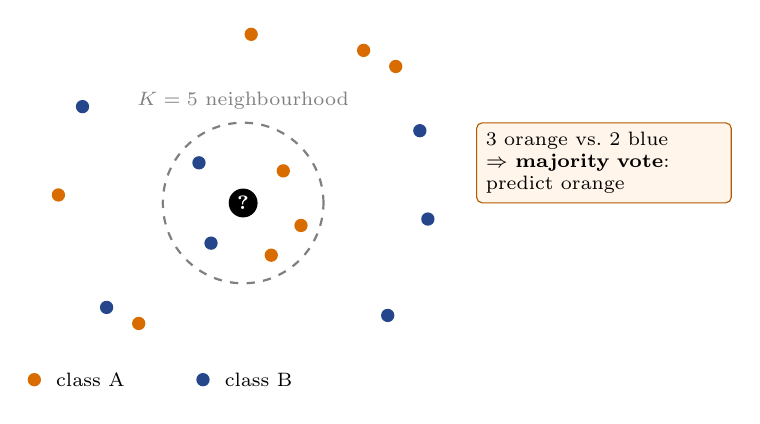
\begin{tikzpicture}[scale=1.02,
     oc/.style={circle,fill=orange!85!black,inner sep=1.7pt},
     bc/.style={circle,fill=accent,inner sep=1.7pt}]
   \node[bc] at (2.2,0.9){}; \node[bc] at (-2.0,1.2){}; \node[bc] at (-1.7,-1.3){};
   \node[bc] at (1.8,-1.4){}; \node[bc] at (2.3,-0.2){};
   \node[oc] at (1.9,1.7){}; \node[oc] at (-2.3,0.1){}; \node[oc] at (0.1,2.1){};
   \node[oc] at (1.5,1.9){}; \node[oc] at (-1.3,-1.5){};
   \node[oc] at (0.5,0.4){}; \node[oc] at (0.35,-0.65){}; \node[oc] at (0.72,-0.28){};
   \node[bc] at (-0.55,0.5){}; \node[bc] at (-0.4,-0.5){};
   \draw[dashed,thick,gray] (0,0) circle (1.0);
   \node[circle,fill=black,text=white,inner sep=1.4pt,font=\scriptsize\bfseries] at (0,0){?};
   \node[font=\scriptsize,text=gray,above] at (0,1.05) {$K=5$ neighbourhood};
   \node[rounded corners=2pt,draw=orange!70!black,fill=orange!8,align=left,font=\scriptsize,text width=3.0cm,anchor=west] at (2.9,0.5) {3 orange vs.\ 2 blue\\$\Rightarrow$ \textbf{majority vote}:\\ predict orange};
   \node[oc] at (-2.6,-2.2){}; \node[right,font=\scriptsize] at (-2.45,-2.2){class A};
   \node[bc] at (-0.5,-2.2){}; \node[right,font=\scriptsize] at (-0.35,-2.2){class B};
  \end{tikzpicture}
  \end{center}
  \begin{takeaway}KNN looks at the $K$ closest training points and predicts their majority class --- here 3 orange beat 2 blue.\end{takeaway}
\end{frame}

\begin{frame}{KNN with $K = 10$ vs.\ Bayes optimum}
  \begin{center}
    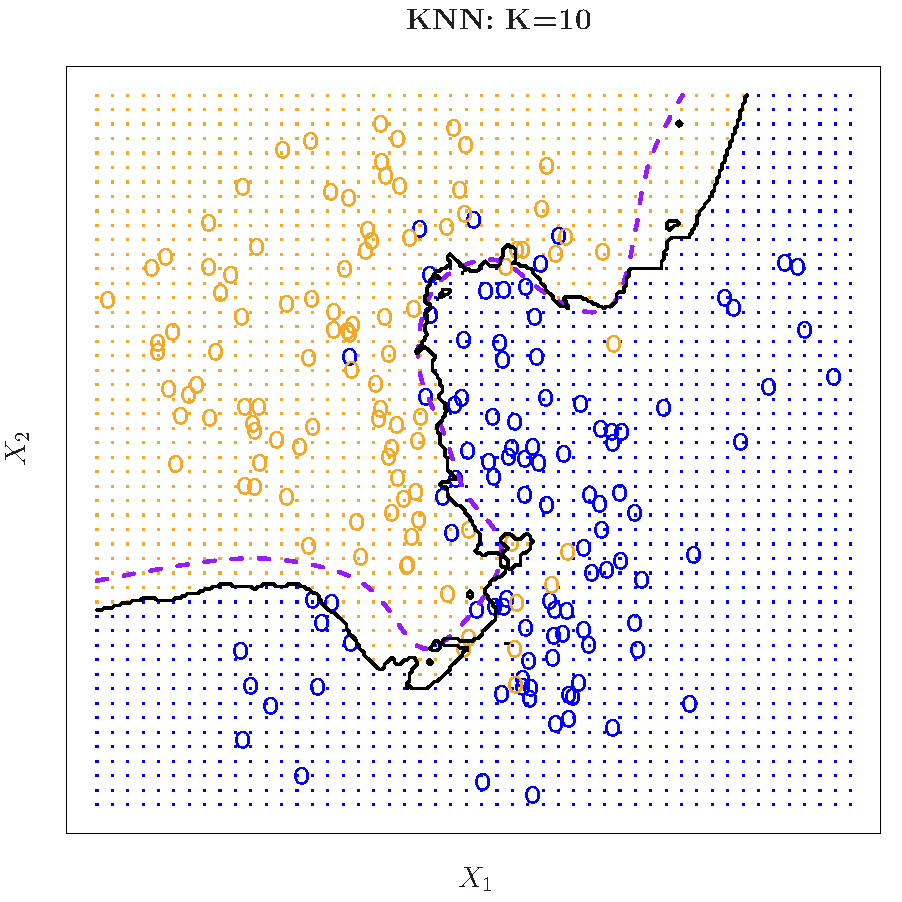
\includegraphics[width=0.85\textwidth,height=0.66\textheight,keepaspectratio]{2_15.pdf}
  \end{center}
  The KNN decision boundary (black) closely follows the Bayes
  boundary (purple dashed) --- with a well-chosen $K$.
  \islpsource{Figure 2.15}
\end{frame}

\begin{frame}{KNN with very small $K$ ($K = 1$)}
  \begin{center}
    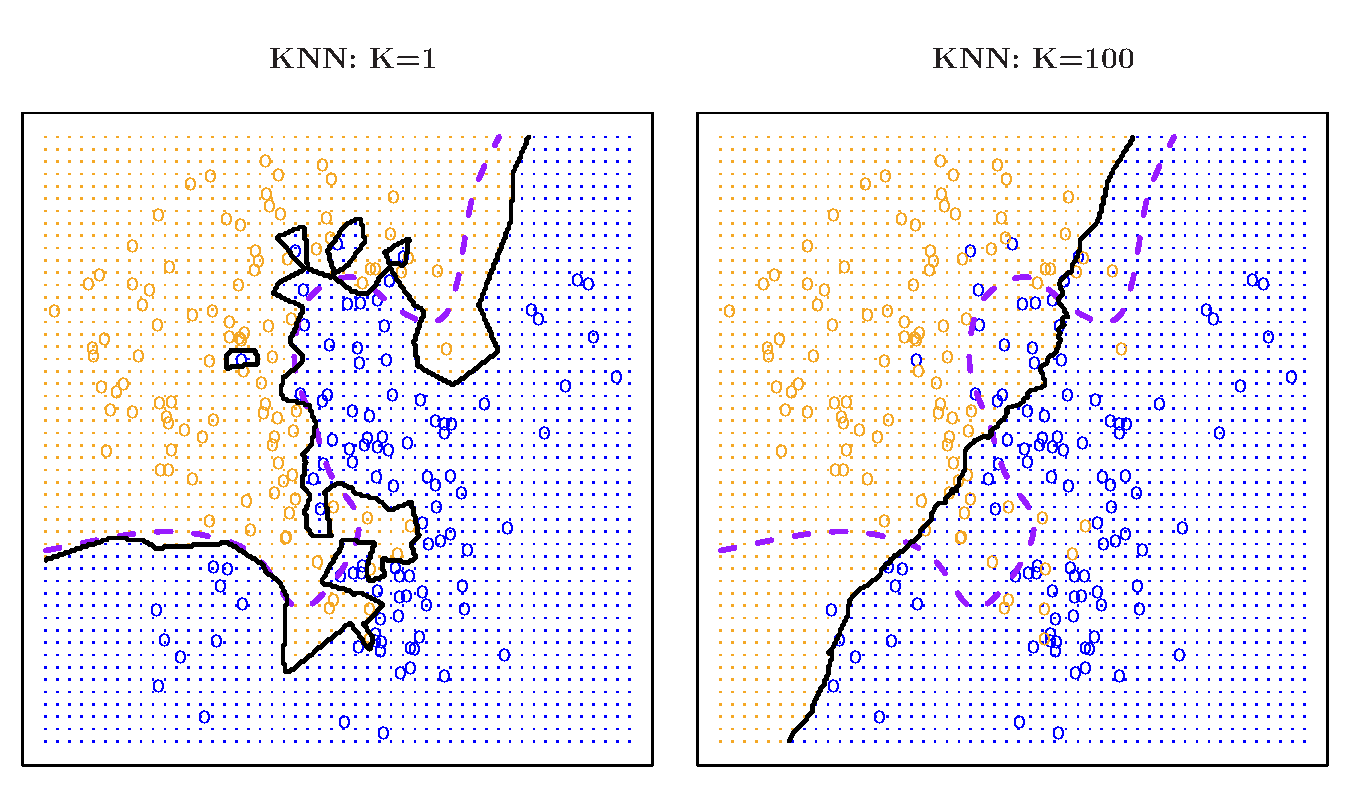
\includegraphics[width=0.85\textwidth,height=0.66\textheight,keepaspectratio]{2_16.pdf}
  \end{center}
  Each training point gets its own little island: the boundary is
  extremely jagged. \emph{Low bias, very high variance} --- training
  error is zero but test error is poor.
  \islpsource{Figure 2.16}
\end{frame}

\begin{frame}{KNN decision boundaries: $K=1$ vs.\ $K=100$}
  \begin{center}
    
\includegraphics[width=0.98\textwidth,height=0.58\textheight,keepaspectratio]{ch02_knn_boundary.png}
  \end{center}
  \begin{takeaway}Small $K$ yields a jagged, high-variance boundary that overfits; large $K$ yields a smooth, high-bias boundary --- the same trade-off, seen geometrically.\end{takeaway}
\end{frame}

\begin{frame}{KNN error vs.\ $1/K$}
  \begin{center}
    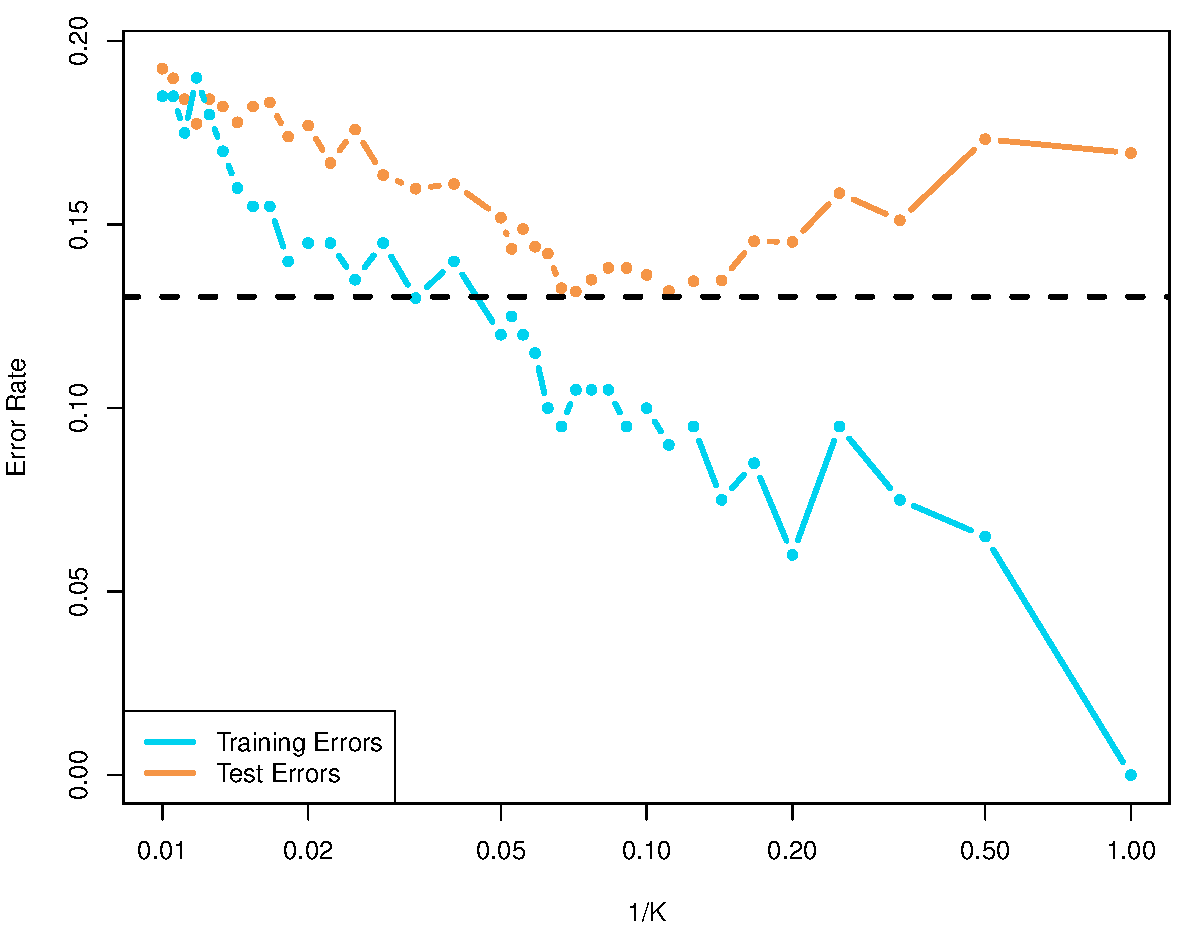
\includegraphics[width=0.85\textwidth,height=0.62\textheight,keepaspectratio]{2_17.pdf}
  \end{center}
  Training error decreases monotonically; test error is U-shaped with
  a minimum at moderate $K$. Cross-validation lets us pick $K$ in
  practice.
  \islpsource{Figure 2.17}
\end{frame}

\begin{frame}{Choosing $K$ in practice}
  \begin{takeaway}[Practical advice]
    \begin{itemize}
      \item Small $K$ $\Rightarrow$ low bias, high variance, jagged
            boundary.
      \item Large $K$ $\Rightarrow$ high bias, low variance, smooth
            boundary.
      \item Try $K \in \{1, 3, 5, 10, 25, 50, 100\}$ and pick by
            cross-validation.
      \item \textbf{Standardise predictors first} --- KNN is sensitive
            to scaling.
    \end{itemize}
  \end{takeaway}
\end{frame}


\begin{frame}{Exercise 2.6 --- Bayes Classifier and Bayes Error Rate [Math]}
\begin{exercise}
A binary problem (classes A, B). $X$ takes three values with the
following marginal and true conditional probabilities:
\begin{center}\footnotesize
\begin{tabular}{cccc}
\toprule
$x$ & $\Pr(X=x)$ & $p_A(x)=\Pr(A\mid x)$ & $p_B(x)=\Pr(B\mid x)$ \\
\midrule
1 & 0.5 & 0.8 & 0.2 \\
2 & 0.3 & 0.4 & 0.6 \\
3 & 0.2 & 0.5 & 0.5 \\
\bottomrule
\end{tabular}
\end{center}
\begin{enumerate}
  \item State the Bayes classifier's prediction at each $x$.
  \item Give the Bayes error at each $x$, $1-\max_k p_k(x)$.
  \item Compute the \emph{overall} Bayes error rate.
  \item Why is the Bayes error rate usually unattainable in practice?
\end{enumerate}
\end{exercise}
\end{frame}

\begin{frame}{Solution --- Exercise 2.6 (1/2)}
\begin{solutionbox}
\textbf{Method.} At each $x$ the Bayes classifier predicts
$\arg\max_k p_k(x)$ --- the majority class among cases with that $x$
--- because any other choice would err more often at that $x$.
\begin{enumerate}
  \item Compare the two conditional probabilities at each $x$:
        $x=1\to$ \textbf{A} ($0.8>0.2$); $x=2\to$ \textbf{B}
        ($0.6>0.4$); $x=3\to$ tie ($0.5/0.5$), predict either --- the
        error is $0.5$ either way.
  \item Local Bayes error $=1-\max_k p_k$, i.e.\ the probability mass
        of the \emph{losing} class: at $x=1$, $1-0.8=0.2$; at
        $x=2$, $1-0.6=0.4$; at $x=3$, $1-0.5=0.5$.
\end{enumerate}
\end{solutionbox}
\end{frame}

\begin{frame}{Solution --- Exercise 2.6 (2/2)}
\begin{solutionbox}
\begin{enumerate}\setcounter{enumi}{2}
  \item The overall error is the \emph{expectation} of the local error
        over the distribution of $X$ (law of total probability), so we
        weight each local error by $\Pr(X=x)$:
        \[
          0.5(0.2)+0.3(0.4)+0.2(0.5)=0.10+0.12+0.10=\mathbf{0.32}.
        \]
        Interpretation: even the \emph{optimal} rule is wrong on
        $32\,\%$ of cases --- the classes overlap heavily, so this is
        an intrinsically hard problem.
  \item It requires the \emph{true} conditional probabilities
        $p_k(x)$, which are unknown; a real classifier only
        \emph{estimates} them from data, so it does at least as badly.
        The Bayes error is the classification analogue of the
        irreducible error $\mathrm{Var}(\varepsilon)$.
\end{enumerate}
\smallskip
{\itshape Common mistake: averaging the three local errors without the
weights, $(0.2+0.4+0.5)/3\approx0.367$ --- wrong, because the three
$x$-values are not equally likely ($x=1$ occurs half the time).}
\end{solutionbox}
\end{frame}

\begin{frame}{Exercise 2.7 --- KNN by Hand, $K=1$ and $K=3$ [Math]}
\begin{exercise}
Six labelled training points in 2-D:
\begin{center}\footnotesize
\begin{tabular}{cccc}
\toprule
Point & $X_1$ & $X_2$ & Class \\
\midrule
$P_1$ & 2 & 4 & Blue \\
$P_2$ & 1 & 2 & Red \\
$P_3$ & 3 & 2 & Red \\
$P_4$ & 4 & 4 & Blue \\
$P_5$ & 1 & 5 & Blue \\
$P_6$ & 4 & 1 & Red \\
\bottomrule
\end{tabular}
\end{center}
Classify the query $x_0=(2,3)$ with Euclidean distance for
\textbf{$K=1$} and \textbf{$K=3$}. Show the distances and the
estimated class probabilities.
\end{exercise}
\end{frame}

\begin{frame}{Solution --- Exercise 2.7 (1/2)}
\begin{solutionbox}
\textbf{Method.} KNN ranks the training points by Euclidean distance
$d=\sqrt{(X_1-2)^2+(X_2-3)^2}$ to the query $x_0=(2,3)$. Because the
square root is monotone, ranking by $d^2$ gives the same neighbours ---
e.g.\ for $P_2(1,2)$: $d^2=(1-2)^2+(2-3)^2=1+1=2$. Squared distances
for all points (then $d=\sqrt{\,\cdot\,}$):
\begin{center}\footnotesize
\begin{tabular}{ccc}
\toprule
Point & $d^2$ & $d$ \\
\midrule
$P_1(2,4)$ & $0+1=1$ & $1.000$ \\
$P_2(1,2)$ & $1+1=2$ & $1.414$ \\
$P_3(3,2)$ & $1+1=2$ & $1.414$ \\
$P_5(1,5)$ & $1+4=5$ & $2.236$ \\
$P_4(4,4)$ & $4+1=5$ & $2.236$ \\
$P_6(4,1)$ & $4+4=8$ & $2.828$ \\
\bottomrule
\end{tabular}
\end{center}
\textbf{$K=1$:} the single nearest neighbour is $P_1$ (Blue) at
$d=1.0$, so $\hat\Pr(\text{Blue})=1$ and we predict \textbf{Blue}.
\end{solutionbox}
\end{frame}

\begin{frame}{Solution --- Exercise 2.7 (2/2)}
\begin{solutionbox}
\textbf{$K=3$:} the three nearest are $P_1$ (Blue), $P_2$ (Red),
$P_3$ (Red). The estimated class probabilities are the vote shares
$\hat\Pr(Y=j\mid X=x_0)=\frac1K\sum_{i\in\mathcal N_0}I(y_i=j)$:
votes Red $=2$, Blue $=1$, so
$\hat\Pr(\text{Red})=\tfrac23$, $\hat\Pr(\text{Blue})=\tfrac13$; we
predict \textbf{Red}.

\textbf{Lesson:} enlarging $K$ averages over a bigger neighbourhood
and can \emph{flip and smooth} the prediction --- here from Blue to
Red. $K=1$ trusts a single point (low bias, high variance); $K=3$
pools three points (more stable, but pulled by farther neighbours).

\smallskip
{\itshape Common mistake: mixing scales when ranking --- comparing one
point's $d^2$ with another point's $d$. Rank every point on the same
scale; $d$ and $d^2$ give the identical ordering, so the square roots
are only needed if the distances themselves are reported.}
\end{solutionbox}
\end{frame}


% ------------------------------------------------------------
% Extended exercises E2.2 (Python) and E2.3 (Math) --- end of KNN section
% ------------------------------------------------------------
\begin{frame}{Extended Exercise 2.2 --- KNN simulation study [Python]}
\begin{longexercise}
Build a controlled experiment that exposes the bias--variance trade-off in KNN.
\begin{enumerate}\setlength\itemsep{1pt}
  \item Simulate a 2-class 2-D problem: class 0 from $\mathcal N((0,0),I)$ and class 1 from $\mathcal N((2,2),I)$. Draw $n_{\text{train}}=200$ and a large $n_{\text{test}}=2000$ (half per class).
  \item For $K=1,2,\ldots,50$ fit a KNN classifier and record the \emph{training} and \emph{test} error rates.
  \item Plot both errors against $1/K$ (flexibility) and identify the $K$ that minimises test error.
  \item Explain each curve via bias and variance, and compare the best test error to the Bayes rate $\Phi(-\sqrt2)\approx0.079$ (means $2\sqrt2$ apart, unit variance).
\end{enumerate}
Provide runnable code and state the expected qualitative result.
\end{longexercise}
\end{frame}

\begin{frame}[fragile]{Solution --- Extended Exercise 2.2 (1/2)}
\begin{solutionbox}
\begin{lstlisting}[basicstyle=\ttfamily\scriptsize]
import numpy as np
from sklearn.neighbors import KNeighborsClassifier
rng = np.random.default_rng(1)                       # seeded RNG (reproducible)
def sample(n):                                       # draw n points, half per class
    n0 = n // 2
    X = np.vstack([rng.normal([0,0], 1, (n0, 2)),    # class 0: centre (0,0)
                   rng.normal([2,2], 1, (n-n0, 2))]) # class 1: centre (2,2)
    return X, np.r_[np.zeros(n0), np.ones(n-n0)]     # features, labels 0/1
Xtr, ytr = sample(200); Xte, yte = sample(2000)      # training and test sets
tr, te = [], []
for K in range(1, 51):                               # fit KNN for K = 1..50
    m = KNeighborsClassifier(K).fit(Xtr, ytr)
    tr.append(1 - m.score(Xtr, ytr)); te.append(1 - m.score(Xte, yte))  # err = 1 - acc
print("best K =", int(np.argmin(te)) + 1, "min test err =", round(min(te), 3))
\end{lstlisting}
\end{solutionbox}
\end{frame}

\begin{frame}[fragile]{Solution --- Extended Exercise 2.2 (2/2)}
\begin{solutionbox}
Plot the two error curves against flexibility $1/K$:
\begin{lstlisting}
import matplotlib.pyplot as plt
inv = [1/K for K in range(1, 51)]   # x-axis: flexibility = 1/K
# draw the training and test error curves on one plot
plt.plot(inv, tr, label="train"); plt.plot(inv, te, label="test")
plt.xlabel("1/K"); plt.ylabel("error rate"); plt.legend(); plt.show()
\end{lstlisting}
\textbf{Expected result (this seed).} Best $K\approx14$ with test error $\approx0.076$ --- essentially the Bayes floor $\approx0.079$.
\begin{itemize}\setlength\itemsep{0pt}
  \item \textbf{Training error} climbs from $0$ at $K=1$ (each point is its own neighbour) to $\approx0.035$; it does \emph{not} track test error.
  \item \textbf{Test error} is U-shaped in $1/K$: worst at $K=1$ ($\approx0.093$, high \emph{variance}), dips near $K\approx10\text{--}20$, then drifts up for very large $K$ (rising \emph{bias}).
\end{itemize}
Small $K$ $=$ flexible $=$ low bias, high variance; large $K$ $=$ rigid $=$ high bias, low variance. Cross-validation would pick $K$ in the flat basin at the bottom.
\end{solutionbox}
\end{frame}

\begin{frame}{Extended Exercise 2.3 --- Bayes boundary for two Gaussians [Math]}
\begin{longexercise}
A 1-D two-class problem with \emph{common}-variance Gaussian class densities:
\[
X\mid Y{=}0\sim\mathcal N(\mu_0,\sigma^2),\qquad X\mid Y{=}1\sim\mathcal N(\mu_1,\sigma^2),
\]
priors $\pi_0=\Pr(Y{=}0)$ and $\pi_1=1-\pi_0$. Use $\mu_0=0$, $\mu_1=2$, $\sigma=1$, $\pi_0=0.6$, $\pi_1=0.4$.
\begin{enumerate}\setlength\itemsep{1pt}
  \item Write the Bayes classifier via the posteriors $\propto\pi_k f_k(x)$.
  \item Taking logs, derive the boundary and show $x^\star=\dfrac{\mu_0+\mu_1}{2}+\dfrac{\sigma^2}{\mu_1-\mu_0}\ln\dfrac{\pi_0}{\pi_1}$; evaluate it.
  \item Compute the Bayes error $\pi_0\Pr(X{>}x^\star\mid Y{=}0)+\pi_1\Pr(X{<}x^\star\mid Y{=}1)$, using $\Phi(1.20)=0.885$ and $\Phi(0.80)=0.788$.
  \item Interpret: which way does raising $\pi_0$ move $x^\star$, and what does the Bayes error represent?
\end{enumerate}
\end{longexercise}
\end{frame}

\begin{frame}{Solution --- Extended Exercise 2.3 (1/2)}
\begin{solutionbox}
\textbf{1. Bayes rule.} The posterior is $\Pr(Y{=}k\mid x)\propto\pi_k f_k(x)$ with $f_k(x)=\frac{1}{\sqrt{2\pi}\,\sigma}\exp\!\big(-\frac{(x-\mu_k)^2}{2\sigma^2}\big)$. Predict class~1 iff $\pi_1 f_1(x)>\pi_0 f_0(x)$.

\textbf{2. Boundary.} Take logs of $\pi_1 f_1(x)=\pi_0 f_0(x)$; the constant $\frac{1}{\sqrt{2\pi}\,\sigma}$ cancels:
\[
\ln\pi_1-\frac{(x-\mu_1)^2}{2\sigma^2}=\ln\pi_0-\frac{(x-\mu_0)^2}{2\sigma^2}.
\]
Multiply by $2\sigma^2$ and expand; the $x^2$ terms cancel (equal variances $\Rightarrow$ a \emph{linear} boundary), giving
\[
2(\mu_1-\mu_0)x-(\mu_1^2-\mu_0^2)=2\sigma^2\ln\frac{\pi_0}{\pi_1}
\;\Rightarrow\;
x^\star=\frac{\mu_0+\mu_1}{2}+\frac{\sigma^2}{\mu_1-\mu_0}\ln\frac{\pi_0}{\pi_1}.
\]
Plug in: $x^\star=1+\tfrac12\ln(1.5)=1+\tfrac12(0.405)=\mathbf{1.203}$.
\end{solutionbox}
\end{frame}

\begin{frame}{Solution --- Extended Exercise 2.3 (2/2)}
\begin{solutionbox}
\textbf{3. Bayes error.} With $\sigma=1$: class~0 is misread when $X>x^\star$, probability $\Pr(Z>1.203)=1-\Phi(1.20)\approx0.115$; class~1 is misread when $X<x^\star$, probability $\Pr(Z<1.203-2)=\Phi(-0.797)=1-\Phi(0.80)\approx0.212$. Weight by the priors:
\[
\text{Bayes error}=0.6(0.115)+0.4(0.212)=0.069+0.085=\mathbf{0.154}.
\]
Even the optimal rule misreads about $15\%$ of cases --- the price of the overlap between the two bells.

\textbf{4. Interpretation.} The boundary sits at the midpoint $1$ only when $\pi_0=\pi_1$. Raising $\pi_0$ makes $\ln(\pi_0/\pi_1)>0$, sliding $x^\star$ \emph{toward the rarer class} ($\mu_1$): we cede more of the line to the commoner class~0. The Bayes error is the \emph{irreducible} classification error --- the analogue of $\mathrm{Var}(\varepsilon)$ in regression --- attainable only with the \emph{true} $\pi_k,f_k$; any estimated classifier does at least as badly.
\end{solutionbox}
\end{frame}


% ============================================================
\section{Python Lab}

\begin{frame}{Python lab --- run it live in the notebook}
  \begin{labnote}[Companion notebook: \texttt{chapter\_02\_lab.ipynb}]
    The code in this section is meant to be \textbf{demonstrated live}. Open the companion Jupyter notebook and run it cell by cell:
    \begin{itemize}
      \item a NumPy and pandas refresher, and plotting;
      \item reproducing the bias--variance figure (Fig.~2.9);
      \item $K$-nearest-neighbours classification.
    \end{itemize}
    Data loads via the \texttt{ISLP} package or the bundled CSV files; the notebook ends with hands-on exercises.
  \end{labnote}
\end{frame}


% ============================================================

\begin{frame}[fragile]{Python lab: setup}
  \begin{lstlisting}
import numpy as np                 # arrays and linear algebra
import pandas as pd                # data frames (tables)
import matplotlib.pyplot as plt    # plotting
from ISLP import load_data         # the book's datasets

rng = np.random.default_rng(2024)  # seeded random generator
plt.rcParams['figure.dpi'] = 110   # sharper inline figures
  \end{lstlisting}
  Always seed your RNG for reproducible plots.
\end{frame}

\begin{frame}[fragile]{NumPy basics}
  \begin{lstlisting}
x = np.array([3, 4, 5])           # 1-D array (a vector)
y = np.array([4, 9, 7])

x.sum(), x.mean(), x.std(ddof=1)  # basic stats (sample sd)
A = np.array([[1, 2], [3, 4]])    # 2 x 2 matrix
A.shape, A.T, np.linalg.inv(A), A @ A  # shape, transpose, inverse, product
  \end{lstlisting}
\end{frame}

\begin{frame}[fragile]{KNN classification}
  \begin{lstlisting}
from sklearn.neighbors import KNeighborsClassifier
from sklearn.model_selection import train_test_split
from sklearn.preprocessing import StandardScaler

Default = load_data("Default")             # credit-card default data
y = (Default["default"] == "Yes").astype(int).values  # 1 = default
X = Default[["balance", "income"]].values  # two numeric predictors
Xtr, Xte, ytr, yte = train_test_split(X, y, test_size=0.3,
                                       random_state=0)  # 70/30 split
scaler = StandardScaler().fit(Xtr)         # KNN needs scaled features
# fit 10-NN on the standardised training data:
knn = KNeighborsClassifier(n_neighbors=10).fit(scaler.transform(Xtr), ytr)
print(knn.score(scaler.transform(Xte), yte))  # test-set accuracy
  \end{lstlisting}
\end{frame}


\begin{frame}{Exercise 2.8 --- Scatter and Flexibility on Auto [Python]}
\begin{exercise}
Load the \texttt{Auto} data, make a scatter plot of \texttt{mpg}
(y-axis) against \texttt{horsepower} (x-axis), and comment on what
level of \emph{flexibility} a good model of this relationship needs.
Note that \texttt{horsepower} contains a few ``\texttt{?}'' missing
entries you must handle.
\end{exercise}
\end{frame}

\begin{frame}[fragile]{Solution --- Exercise 2.8 (1/2)}
\begin{solutionbox}
\begin{lstlisting}
import pandas as pd
import matplotlib.pyplot as plt

Auto = pd.read_csv("../../ALL CSV FILES - 2nd Edition/Auto.csv")
Auto = Auto[Auto["horsepower"] != "?"].copy()   # drop 5 missing
Auto["horsepower"] = Auto["horsepower"].astype(float)  # str -> num

plt.scatter(Auto["horsepower"], Auto["mpg"], s=10)  # small dots
plt.xlabel("horsepower"); plt.ylabel("mpg")
plt.show()

print(Auto.shape[0])                              # 392
print(Auto["horsepower"].corr(Auto["mpg"]))       # about -0.78
\end{lstlisting}
\end{solutionbox}
\end{frame}

\begin{frame}{Solution --- Exercise 2.8 (2/2)}
\begin{solutionbox}
\textbf{Interpretation.} After dropping the 5 missing rows, $n=392$.
The cloud is clearly \emph{nonlinear}: \texttt{mpg} falls steeply as
\texttt{horsepower} rises and then flattens (a convex, decreasing
curve; correlation $\approx-0.78$). A straight-line fit would
\emph{underfit} this curvature (high bias); a \emph{moderately}
flexible fit --- a quadratic/polynomial or a spline --- captures it
well; an extremely flexible fit that wiggles through every point would
\emph{overfit} (high variance).

\textbf{Why the cleaning steps matter.} The ``\texttt{?}'' entries make
pandas read \texttt{horsepower} as \emph{strings} (dtype
\texttt{object}); the filter removes those rows and
\texttt{astype(float)} restores a numeric column --- only then are the
scatter plot, the correlation, and any later fit meaningful.

\smallskip
{\itshape Common mistake: skipping the conversion (the correlation
fails or is computed on nonsense) --- and note that a strong
correlation does \emph{not} certify a linear fit: $-0.78$ measures
linear association, yet the visible curvature still calls for a
nonlinear term.}
\end{solutionbox}
\end{frame}


% ------------------------------------------------------------
% Extended exercise E2.4 (Integrative) --- end of Python Lab section
% ------------------------------------------------------------
\begin{frame}{Extended Exercise 2.4 --- Linear vs KNN: which wins when? [Integrative]}
\begin{longexercise}
Six 1-D training points $(x,y)$:
\[
(1,1.0)\ (2,1.8)\ (3,3.3)\ (4,3.9)\ (5,5.2)\ (6,5.8).
\]
An OLS line fitted to them is $\hat y=0.02+0.994\,x$. Query point $x_0=3.2$.
\begin{enumerate}\setlength\itemsep{1pt}
  \item \textbf{KNN regression by hand.} List the distances $|x_i-x_0|$; predict $\hat y(x_0)$ for $K=1$ and $K=3$ (a KNN regressor \emph{averages} the $K$ nearest responses).
  \item Predict $\hat y(x_0)$ from the linear model. Are the three predictions close here, and why?
  \item For each case name the expected winner (parametric \emph{linear} vs nonparametric \emph{KNN}) with a reason: (a) true $f$ linear; (b) true $f$ strongly nonlinear with large $n$; (c) $p$ large (say $20$) with modest $n$.
  \item Give a one-sentence rule of thumb for choosing between them.
\end{enumerate}
\end{longexercise}
\end{frame}

\begin{frame}{Solution --- Extended Exercise 2.4 (1/2)}
\begin{solutionbox}
\textbf{1. KNN by hand} at $x_0=3.2$ (points sorted by distance):
\begin{center}\footnotesize
\begin{tabular}{lcccccc}
\toprule
$x_i$        & 3   & 4   & 2   & 5   & 1   & 6   \\
$|x_i-x_0|$  & 0.2 & 0.8 & 1.2 & 1.8 & 2.2 & 2.8 \\
$y_i$        & 3.3 & 3.9 & 1.8 & 5.2 & 1.0 & 5.8 \\
\bottomrule
\end{tabular}
\end{center}
$K=1$: nearest is $x=3$, so $\hat y(x_0)=3.3$. \quad
$K=3$: nearest are $x=3,4,2$ with $y=3.3,3.9,1.8$, so $\hat y(x_0)=\tfrac{3.3+3.9+1.8}{3}=3.0$.

\textbf{2. Linear model.} $\hat y(x_0)=0.02+0.994(3.2)=3.20$. All three ($3.30$, $3.00$, $3.20$) are close \emph{because the data are nearly linear}: a global line and a local average agree when $f$ is smooth and roughly straight. ($K=3$ dips a little, pulled down by the far point $x=2$.)
\end{solutionbox}
\end{frame}

\begin{frame}{Solution --- Extended Exercise 2.4 (2/2)}
\begin{solutionbox}
\textbf{3. Who wins in general?}
\begin{itemize}\setlength\itemsep{1pt}
  \item \textbf{(a) True $f$ linear $\Rightarrow$ linear wins.} It is correctly specified (no bias) and low-variance (few parameters, uses all $n$ points); KNN only adds variance by averaging $K$ local points and is biased near the edges.
  \item \textbf{(b) Strongly nonlinear $f$, large $n$ $\Rightarrow$ KNN wins.} The linear model carries irremovable \emph{misspecification bias}; with large $n$ the neighbourhoods are dense, so KNN's variance is small and its flexibility captures the curvature.
  \item \textbf{(c) Large $p$ ($\approx20$), modest $n$ $\Rightarrow$ linear wins.} \emph{Curse of dimensionality}: in high dimensions the ``nearest'' neighbours are actually far, so KNN averages dissimilar points. A parametric model that assumes structure is far more data-efficient.
\end{itemize}
\textbf{4. Rule of thumb.} Prefer nonparametric KNN when $f$ is unknown/curved, $p$ is small, and $n$ is large; prefer the parametric linear model when $n$ is small, $p$ is large, the functional form is trustworthy, or you need interpretability.
\end{solutionbox}
\end{frame}


% ============================================================
\section{Summary}
% ============================================================

\begin{frame}{Chapter 2 in one slide}
  \begin{block}{What we accomplished}
    Established the formal framework: the unknown $f$, irreducible
    error $\varepsilon$, and the core trade-offs.
  \end{block}
  \begin{itemize}
    \item Decomposed prediction error into reducible + irreducible.
    \item Compared parametric (linear) and nonparametric (smooth
          spline) fits.
    \item Showed why test MSE has a U-shape (bias-variance).
    \item Defined the Bayes classifier and the Bayes error rate.
    \item Met our first method: $K$-nearest neighbours.
  \end{itemize}
\end{frame}

\begin{frame}{Key formulas at a glance}
  \footnotesize
  \begin{description}
    \item[Model] $Y=f(X)+\varepsilon$, \quad $E[\varepsilon]=0$, \ $\operatorname{Var}(\varepsilon)=\sigma^2$.
    \item[Error split] $E[(Y-\hat f)^2]=\underbrace{[f-\hat f]^2}_{\text{reducible}}+\underbrace{\sigma^2}_{\text{irreducible}}$.
    \item[Test MSE] $\dfrac1n\sum_{i=1}^n\big(y_i-\hat f(x_i)\big)^2$.
    \item[Bias--variance] $E\big[(y_0-\hat f(x_0))^2\big]=\operatorname{Var}(\hat f(x_0))+\big[\operatorname{Bias}(\hat f(x_0))\big]^2+\sigma^2$.
    \item[Bayes rule] assign $x_0$ to $\arg\max_j \Pr(Y=j\mid X=x_0)$; \ Bayes error $=1-E\big[\max_j \Pr(Y=j\mid X)\big]$.
    \item[KNN] $\Pr(Y=j\mid X=x_0)=\dfrac1K\sum_{i\in\mathcal N_0} I(y_i=j)$.
  \end{description}
\end{frame}

\begin{frame}{Vocabulary checklist}
  \footnotesize
  \begin{tabular}{ll}
    \toprule
    \textbf{Term} & \textbf{Meaning} \\
    \midrule
    $f(X)$ & Systematic part of $Y$ given $X$ \\
    $\varepsilon$ & Irreducible noise; $\mathrm{Var}(\varepsilon) = \sigma^2$ \\
    Reducible / irreducible error & Comes from $\hat f$ / from $\varepsilon$ \\
    Parametric / nonparametric & Fixed-form $f$ / data-driven $f$ \\
    Flexibility & Effective number of parameters \\
    Training MSE / test MSE & On train data / on held-out data \\
    Bias / variance / irreducible error & Three parts of expected test MSE \\
    Overfitting / underfitting & High variance / high bias \\
    Bayes classifier / Bayes error & Optimal classifier / its error rate \\
    KNN & Local-majority classifier with $K$ neighbours \\
    \bottomrule
  \end{tabular}
\end{frame}

\begin{frame}{Decision rules of thumb}
  \begin{block}{Choosing flexibility}
    \begin{itemize}
      \item Small $n$, simple-looking data $\Rightarrow$ low
            flexibility wins.
      \item Large $n$, complex truth $\Rightarrow$ high flexibility
            wins.
      \item Inference goal $\Rightarrow$ pay an interpretability
            premium for low flexibility.
      \item Pure prediction $\Rightarrow$ choose by cross-validated
            test error.
    \end{itemize}
  \end{block}
\end{frame}

\begin{frame}{Common pitfalls}
  \begin{alertblock}{Watch out for}
    \begin{enumerate}
      \item Comparing methods on training MSE.
      \item Using KNN without standardising features.
      \item Reporting accuracy on imbalanced classes.
      \item Confusing the curse of dimensionality with simply ``a lot
            of data'' --- both can hurt KNN.
      \item Treating the Bayes classifier as something you can fit
            (you can't).
      \item Forgetting that bias and variance are computed over many
            training sets.
    \end{enumerate}
  \end{alertblock}
\end{frame}

\begin{frame}{Self-check questions}
  \begin{enumerate}
    \item Sketch the bias-variance decomposition curves. Where is the
          optimal flexibility?
    \item Why is the irreducible error not a function of $\hat f$?
    \item Construct an example where a more flexible method is
          preferable to a linear model.
    \item For KNN, what happens to bias and variance as $K$ grows?
    \item State the Bayes classifier in words; why is it the gold
          standard?
    \item Suppose you have $n = 50$ observations of $p = 1$ predictor
          and want to estimate $E[Y \mid X]$. Pick a method and
          justify.
  \end{enumerate}
\end{frame}

\begin{frame}{Ten things to remember}
  \begin{enumerate}
    \item $Y = f(X) + \varepsilon$: $f$ is what we estimate.
    \item Reducible vs.\ irreducible error.
    \item Two goals: prediction and inference.
    \item Two strategies: parametric vs.\ nonparametric.
    \item Flexibility vs.\ interpretability trade-off.
    \item Training MSE is too optimistic --- only test MSE matters.
    \item Bias-variance: $E[(y_0 - \hat f)^2] = \mathrm{Bias}^2 +
          \mathrm{Var}(\hat f) + \sigma^2$.
    \item Optimal flexibility minimises the U-shape of test MSE.
    \item Bayes classifier is the gold standard; Bayes error is the
          floor.
    \item KNN: simple, flexible, sensitive to $K$ and to scaling.
  \end{enumerate}
\end{frame}

\begin{frame}{What's next}
  Chapter 3: \emph{Linear Regression}.
  \begin{itemize}
    \item The simplest --- and still most-used --- statistical learning
          method.
    \item Fit, interpret, quantify uncertainty, diagnose problems.
    \item The benchmark against which every fancier method gets
          compared.
  \end{itemize}
\end{frame}

\end{document}
